\documentclass[a4paper,12pt]{article}
\usepackage[utf8]{inputenc}
\usepackage[ngerman]{babel}
\usepackage[T1]{fontenc}
\usepackage{amsmath}
\usepackage{amssymb}
\usepackage{amsthm}
\usepackage{geometry}
\usepackage{graphicx}
\usepackage{xcolor}
\definecolor{darkblue}{RGB}{0,0,139}
\usepackage[colorlinks=true,linkcolor=darkblue,citecolor=darkblue,urlcolor=darkblue]{hyperref}
\usepackage{pgfplots}
\usepackage{float}
\usepackage{booktabs}
\usepackage{listings}
\usepackage{rotating}
\usepackage{adjustbox}
\usepackage{enumitem}
\setlist[itemize]{label=-}
\usepackage[protrusion=true,expansion=true,final]{microtype}
\usepackage{url}
\urlstyle{same}
% Prevent text overflow beyond right DIN A4 margin
\sloppy
\emergencystretch=3em

\pgfplotsset{compat=1.18}

\geometry{margin=2.5cm}

\theoremstyle{definition}
\newtheorem{definition}{Definition}
\newtheorem{bemerkung}{Bemerkung}
\newtheorem{beispiel}{Beispiel}
\newtheorem{satz}{Satz}
\newtheorem{lemma}{Lemma}
\newtheorem{korollar}{Korollar}
\newtheorem{hypothese}{Hypothese}
\newtheorem{beobachtung}{Beobachtung}

% Code-Listing Style
\lstdefinestyle{pythonstyle}{
    language=Python,
    basicstyle=\ttfamily\small,
    keywordstyle=\color{blue},
    commentstyle=\color{gray},
    stringstyle=\color{red},
    numbers=left,
    numberstyle=\tiny\color{gray},
    stepnumber=1,
    numbersep=5pt,
    backgroundcolor=\color{white},
    showspaces=false,
    showstringspaces=false,
    showtabs=false,
    frame=single,
    tabsize=2,
    captionpos=b,
    breaklines=true,
    breakatwhitespace=false,
    escapeinside={\%*}{*)},
}

\title{Phi-Navigation für Roboter\\
	\large Lokale Wegplanung nach goldenem Schnitt}

\author{Stephan Epp}
\date{\today}

\begin{document}
	
\maketitle
\tableofcontents
\newpage

\section{Einführung}
Die Motivation und Überzeugung für diese Arbeit ist grundlegend durch die Beschreibung des folgenden Modells für Roboter geprägt.

\begin{definition}[Lokale Robotermodell]
Das lokale Robotermodell besteht darin:
\begin{enumerate}
	\item Die Planung für Wege und die Ausführung von Plänen der sRoboter erfolgt nur in ihrer lokalen Umgebung.
	\item Die Planung für Wege für entfernte Ziele erfolgt der lokalen Richtung nach immer konkreter, bis das Ziel erreicht ist. Den ganzen optimalen Weg kennt der Roboter zu Beginn nicht. Er kennt immer nur die richtige Richtung in seiner lokalen Umgebung.
\end{enumerate}	
\end{definition}

Dieses grundlegende und natürliche Prinzip, welches dem Roboter alle Bewegungsfreiheiten gibt, trifft die Realität am besten. Es kommt der natürlichen e-Funktion, der Energiefunktion, am nächsten. Der Roboter ist vergleichbar mit einem dynamischen System. Und erst so trifft der Roboter als dynamisches System in seiner charakteristischen Beschreibung das Optimum mit dem goldenen Schnitt \cite{phi_energy}. Der Roboter ist vergleichbar mit einer Arbeitsbiene, die dem Roboter ein Vorbild in der Arbeitsweise gibt.

Die autonome Navigation mobiler Roboter ist eine zentrale Herausforderung der modernen Robotik. Klassische Ansätze wie A*-Algorithmus, RRT (Rapidly-exploring Random Trees) oder Dijkstra basieren auf globaler Wegplanung mit vollständiger Kartierung der Umgebung. Diese Methoden erfordern erhebliche Rechenressourcen und sind anfällig gegenüber Umgebungsänderungen.

Die Natur hingegen zeigt uns alternative Strategien: Bienen navigieren zu Futterquellen ohne globale Karten, nur mit lokalen Entscheidungen. Sie erreichen ihre Ziele energieeffizient und robust. Diese Arbeit überträgt Prinzipien aus der natürlichen Navigation und der Theorie energieoptimaler dynamischer Systeme auf die Robotik.

\subsection{Der goldene Schnitt in dynamischen Systemen}

Der goldene Schnitt $\phi = \frac{1+\sqrt{5}}{2} \approx 1{,}618033989$ ist nicht nur eine geometrische Konstante, sondern – wie in \cite{phi_energy} gezeigt – der optimale Exponent für Energiefunktionen schwerpunktorientierter dynamischer Systeme:

\begin{equation}
E_{\text{optimal}}(t) = E_0 \cdot e^{-\phi t}
\end{equation}

Diese Erkenntnis bildet die theoretische Grundlage für eine neue Klasse von Navigationsalgorithmen, bei denen Roboter als energiedissipierende dynamische Systeme betrachtet werden.

\subsection{Phi-Navigation}

\begin{satz}[Phi-Navigation]
	Ein mobiler Roboter, der ausschließlich auf Basis lokaler Informationen navigiert und dessen Geschwindigkeitsprofil dem $\phi$-exponentiellen Energieabfall folgt, erreicht optimale Navigation im Sinne von:
	\begin{enumerate}
		\item[-] Minimaler Energiedissipation
		\item[-] Maximaler Robustheit gegenüber Umgebungsänderungen
		\item[-] Natürlichem, bioinspiriertem Bewegungsmuster
		\item[-] Geringem Rechenaufwand
	\end{enumerate}
\end{satz}

\begin{proof}[Beweis]
	Wir zeigen die vier genannten Eigenschaften für einen Roboter, der gemäß dem $\phi$-exponentiellen Geschwindigkeitsprofil $v(d) = v_{\max}(1 - e^{-\phi d/d_{\text{ref}}})$ navigiert und ausschließlich lokale Informationen nutzt:
	\begin{enumerate}
		\item \textbf{Minimale Energiedissipation:} Die Gesamtenergie $E$ ergibt sich durch Integration der Leistungsaufnahme $P = Fv$ über die Zeit. Für das $\phi$-Profil ergibt sich (vgl. \cite{phi_energy}):
		\[
		E = \int_0^\infty P(t)\,dt = \int_0^\infty F v(t)\,dt
		\]
		Da $v(t)$ exponentiell mit $\phi$ abklingt, ist $E$ für $\phi$ minimal, da $\phi$ das optimale Verhältnis zwischen schneller Annäherung und sanftem Auslaufen darstellt.
		\item \textbf{Maximale Robustheit:} Die Navigation basiert nur auf aktuellen Sensordaten. Änderungen in der Umgebung werden sofort erkannt und führen zu einer lokalen Anpassung der Trajektorie. Es gibt keine Abhängigkeit von globalen Karten oder Vorwissen, wodurch der Roboter robust gegenüber unerwarteten Hindernissen und Veränderungen bleibt.
		\item \textbf{Natürliches Bewegungsmuster:} Das $\phi$-Profil entspricht dem Energieabfall in natürlichen Systemen (z.B. Bienenflug, biologische Dämpfung). Die resultierenden Trajektorien sind glatt, kontinuierlich und wirken für Beobachter organisch und vorhersehbar.
		\item \textbf{Geringer Rechenaufwand:} Die Berechnung der Steuerbefehle erfolgt ausschließlich auf Basis lokaler Sensorwerte und einfacher mathematischer Operationen (Exponentialfunktion, Addition, Multiplikation). Es sind keine komplexen Planungsalgorithmen oder große Datenstrukturen erforderlich. Die Rechenzeit pro Schritt ist konstant ($O(1)$).
	\end{enumerate}
	Damit sind alle vier Eigenschaften für die Phi-Navigation erfüllt.
\end{proof}

\subsection{Struktur der Arbeit}

Die Arbeit ist wie folgt aufgebaut:
\begin{itemize}
	\item \textbf{Kapitel 2} entwickelt die mathematischen und physikalischen Grundlagen, beschreibt das Robotermodell, das Energiemodell und das lokale Navigationsmodell.
	\item \textbf{Kapitel 3} beschreibt die Simulationsplattform: Software-Architektur, Simulationsumgebung und deren Aufbau.
	\item \textbf{Kapitel 4} erläutert den Phi-Navigationsalgorithmus im Detail, beschreibt die einzelnen Komponenten (Geschwindigkeitsregelung, Hindernisvermeidung, Escape-Mechanismus, Stuck-Erkennung) und deren Zusammenspiel.
	\item \textbf{Kapitel 5} vergleicht die Phi-Navigation mit klassischen Methoden wie A* und RRT sowie mit hybriden Ansätzen und diskutiert die jeweiligen Vor- und Nachteile.
	\item \textbf{Kapitel 6} behandelt die Hardware-Implementierung, insbesondere die Umsetzung auf Mikrocontrollern, die Anforderungen an Sensorik und Aktorik sowie die Positionsschätzung.
	\item \textbf{Kapitel 7} analysiert die Eigenschaften der Phi-Navigation hinsichtlich Konvergenz, Energieoptimalität und Robustheit.
	\item \textbf{Kapitel 8} liefert eine kritische Analyse zentralisierter Navigationsmodelle, diskutiert Limitationen klassischer Ansätze sowie wirtschaftliche und philosophische Konsequenzen.
	\item \textbf{Kapitel 9} fasst die Ergebnisse zusammen, leitet Konsequenzen für Forschung und Industrie ab und gibt einen Ausblick auf zukünftige Arbeiten.
\end{itemize}

\section{Mathematische Grundlagen}

\subsection{Robotermodell}

Wir betrachten einen differentialgetriebenen mobilen Roboter mit Zustand $\mathbf{q}(t) = (x, y, \theta)^T$, wobei $(x,y)$ die Position und $\theta$ die Orientierung im globalen Koordinatensystem darstellt.

\begin{definition}[Differential Drive Kinematik]
	Die Bewegungsgleichungen des Roboters sind gegeben durch:
	\begin{align}
		\dot{x} &= v \cos(\theta) \\
		\dot{y} &= v \sin(\theta) \\
		\dot{\theta} &= \omega
	\end{align}
	mit linearer Geschwindigkeit $v$ und Winkelgeschwindigkeit $\omega$, die aus den Radgeschwindigkeiten $v_L$ und $v_R$ folgen:
	\begin{align}
		v &= \frac{v_R + v_L}{2} \\
		\omega &= \frac{v_R - v_L}{L}
	\end{align}
	wobei $L$ der Radabstand ist.
\end{definition}

\subsection{Energiemodell}

Die kinetische Energie des Roboters ist:

\begin{equation}
E_{\text{kin}} = \frac{1}{2}m v^2 + \frac{1}{2}I \omega^2
\end{equation}

Für ein energieoptimales System mit $\phi$-Dissipation gilt:

\begin{equation}
E(t) = E_0 \cdot e^{-\phi t}
\end{equation}

Dies impliziert für die Geschwindigkeit in Abhängigkeit von der Distanz $d$ zum Ziel:

\begin{equation}\label{eq:phi_speed}
v(d) = v_{\max} \cdot \left(1 - e^{-\phi \cdot d / d_{\text{ref}}}\right)
\end{equation}

wobei $d_{\text{ref}}$ eine Referenzdistanz zur Normalisierung ist.

\subsection{Lokales Navigationsmodell}

\begin{definition}[Lokaler Horizont]
	Der Roboter besitzt einen begrenzten Wahrnehmungshorizont $h_{\text{local}}$. Nur Informationen innerhalb dieses Radius beeinflussen Entscheidungen direkt.
\end{definition}

Dies modelliert die begrenzte Sensorreichweite und entspricht dem natürlichen Verhalten von Lebewesen.

\begin{definition}[Lokales Potentialfeld]
	Das lokale Navigationspotential setzt sich zusammen aus:
	\begin{equation}
		\Phi_{\text{total}}(\mathbf{q}) = \Phi_{\text{attr}}(\mathbf{q}) + \sum_i \Phi_{\text{rep},i}(\mathbf{q})
	\end{equation}
	mit:
	\begin{itemize}
		\item[-] Attraktionspotential zum Ziel: $\Phi_{\text{attr}}$
		\item[-] Repulsionspotentiale von Hindernissen: $\Phi_{\text{rep},i}$
	\end{itemize}
\end{definition}

Die Phi-Gewichtung erfolgt durch:

\begin{equation}
\Phi_{\text{rep}}(d) = \begin{cases}
\frac{\phi}{d} & \text{falls } d < h_{\text{local}} \\
0 & \text{sonst}
\end{cases}
\end{equation}

\subsection{Bienen-Navigation: Biologisches Vorbild}

Honigbienen (Apis mellifera) zeigen bemerkenswerte Navigationsfähigkeiten:

\begin{itemize}
	\item[-] \textbf{Landmark-Navigation}: Orientierung an visuellen Merkmalen
	\item[-] \textbf{Pfadintegration}: Odometrie durch Messung zurückgelegter Strecken
	\item[-] \textbf{Spiralsuche}: Bei Zielannäherung kreisförmiges Absuchen
	\item[-] \textbf{Goldener Winkel}: Optimale Raumabdeckung durch $360^\circ/\phi^2 \approx 137{,}5^\circ$
\end{itemize}

\begin{satz}[Optimaler Explorationswinkel]
	Der goldene Winkel $\alpha = \frac{2\pi}{\phi^2}$ maximiert die räumliche Abdeckung bei sequentiellen Suchschritten.
\end{satz}

\begin{proof}
Der goldene Winkel $\alpha = \frac{2\pi}{\phi^2} \approx 137{,}5^\circ$ ist in der Natur als optimaler Winkel für die Anordnung von Blättern, Samen und anderen Strukturen bekannt. Diese Anordnung, die als Phyllotaxis bezeichnet wird, sorgt dafür, dass sich die einzelnen Elemente möglichst gleichmäßig verteilen und keine Überlappungen entstehen.

Im Kontext der Exploration bedeutet dies: Wenn ein Roboter bei jedem Suchschritt seine Richtung um den goldenen Winkel verändert, werden die Suchpunkte so verteilt, dass sie den Raum maximal abdecken und sich möglichst wenig überschneiden. Mathematisch lässt sich dies dadurch begründen, dass der goldene Winkel irrational ist und somit keine periodische Überlagerung der Suchrichtungen entsteht. Dadurch werden die Suchpunkte gleichmäßig auf dem Kreis verteilt.

Die dichteste Packung von Kreisen, wie sie in der Phyllotaxis-Theorie beschrieben wird, zeigt, dass die Wahl des goldenen Winkels zu einer optimalen Abdeckung führt. Dies wurde in \cite{livio} ausführlich dargestellt und ist in zahlreichen biologischen Systemen beobachtbar. Daher maximiert der goldene Winkel die räumliche Abdeckung bei sequentiellen Explorationsschritten.
\end{proof}

\section{Simulationsplattform}

Diese Kapitel beschreibt den strukturellen Aufbau der Simulationsplattform für Roboter und die Implementierung.

\subsection{Software-Architektur}

Der strukturelle Entwurf der Simulationsplattform für Roboter folgt einem mehrschichtigen Ansatz. Die UML-Diagramme wurden automatisch mit \texttt{pyreverse} aus dem Quellcode generiert und spiegeln die aktuelle Implementierung wider. 

Die Roboter Simulationsplattform ist modular aufgebaut und besteht aus mehreren Schichten, die jeweils spezifische Aufgaben übernehmen. 
\begin{figure}[h]
	\centering
	
\includegraphics[width=1.0\textwidth]{../doc/uml/packages_robosim.pdf}
	\caption{UML-Paketdiagramm der Simulationsplattform}
	\label{fig:uml_packages}
\end{figure}
Die folgende Abbildung \ref{fig:uml_packages} zeigt die Architektur. Das Paketdiagramm verdeutlicht die Beziehungen zwischen den Hauptmodulen

\begin{itemize}
	\item[-] \textbf{src.robot\_core}: Basis-Controller und Steuerlogik
	\item[-] \textbf{src.phi.phi\_navigation}: Phi-Navigationsalgorithmus
	\item[-] \textbf{src.sim.simulation\_engine}: Physik und Umgebung
	\item[-] \textbf{src.sim.simulation\_gui}: Visualisierung und Bedienung
	\item[-] \textbf{src.command\_demo}, \textbf{src.microcontroller\_example}: Demo und Hardwareintegration
\end{itemize}

\begin{sidewaysfigure}
	\centering
	
\includegraphics[width=\textwidth,angle=0,origin=c]{../doc/uml/classes_robosim.pdf}
	\caption{UML-Klassendiagramm der Simulationsplattform}
	\label{fig:uml_classes}
\end{sidewaysfigure}

Das Klassendiagramm \ref{fig:uml_classes} zeigt die wichtigsten Klassen und deren Beziehungen. Die Klasse \texttt{SimulationEngine} verwaltet die Umgebung und die Roboter, die \texttt{RobotController} steuert die Bewegung, und der \texttt{PhiNavigationController} implementiert den Algorithmus zur Phi-Navigation. Die GUI-Komponenten ermöglichen die Visualisierung und Interaktion.

\subsection{Clean Architecture und SOLID-Prinzipien}

Die Implementierung folgt konsequent den SOLID-Prinzipien der objektorientierten Programmierung:

\begin{itemize}
	\item \textbf{Single Responsibility}: Jede Klasse hat genau eine Verantwortung, zum Beispiel \texttt{PhiNavigationController} nur für Navigation, \texttt{SimulationEngine} nur für die Physik
	
	\item \textbf{Open/Closed}: Klassen sind offen für Erweiterung (neue Controller durch Vererbung), aber geschlossen für Modifikation (Basisklasse bleibt stabil)
	
	\item \textbf{Liskov Substitution}: Alle Controller-Subklassen können verwendet werden, wo \texttt{RobotController} erwartet wird
	
	\item \textbf{Interface Segregation}: Abstrakte Methoden \texttt{\_compute\_local\_goal\_direction()} und \texttt{\_estimate\_distance\_to\_goal()}
	
	\item \textbf{Dependency Inversion}: Abhängigkeiten zeigen auf Abstraktionen, nicht auf Konkretisierungen wie zum Beispiel der \texttt{RobotController}
\end{itemize}

\begin{table}[H]
	\centering
	\caption{Code-Metriken der Implementierung}
	\label{tab:code_metrics}
	\begin{tabular}{lrrr}
		\toprule
		\textbf{Modul} & \textbf{Zeilen} & \textbf{Klassen} & \textbf{Abhängigkeiten} \\
		\midrule
		robot\_core.py & 320 & 7 & 0 (Standard-Lib only) \\
		phi\_navigation.py & 406 & 2 & 1 (robot\_core) \\
		phi\_navigation\_sim.py & 160 & 3 & 2 (phi\_nav, robot\_core) \\
		simulation\_engine.py & 280 & 8 & 1 (robot\_core) \\
		simulation\_gui.py & 340 & 3 & 3 (Qt, engine, robot\_core) \\
		\midrule
		\textbf{Gesamt} & \textbf{1506} & \textbf{23} & \textbf{Minimal} \\
		\bottomrule
	\end{tabular}
\end{table}

\subsubsection{Details zur Architektur}

\paragraph{Schicht 1: Wiederverwendbare Controller}

Die unterste Schicht (\texttt{robot\_core}) enthält ausschließlich Python-Standard-Bibliotheken und ist vollständig MicroPython-kompa\-tibel. Diese Schicht umfasst:

\begin{itemize}
	\item \textbf{RobotController}: Abstrakte Basisklasse für alle Verhaltensweisen mit Template Method Pattern
	\item \textbf{PhiNavigationController}: Kernimplementierung der $\phi$-basierten Navigation
	\item \textbf{BeeNavigationController}: Erweiterte Navigation mit Spiralsuche am Ziel
	\item \textbf{MultiGoalPhiNavigator}: Wegpunkt-basierte Navigation für Sammelaufgaben
	\item \textbf{RobotState}: Zustandsrepräsentation (Position, Orientierung, Geschwindigkeiten)
	\item \textbf{SensorData}: Abstraktion von Sensormessungen
\end{itemize}

\textbf{Kritisches Designprinzip:} Diese Module haben \emph{keine Abhängigkeiten} zu Qt, NumPy, PyQt oder anderen Simulations-spezifischen Bibliotheken. Der gesamte Code kann ohne Modifikation auf Mikrocontroller wie ESP32 oder Raspberry Pi Pico kopiert und ausgeführt werden.

\begin{lstlisting}[style=pythonstyle, caption={Abstrakte Basisklasse für maximale Wiederverwendbarkeit}]
class RobotController:
    """Basisklasse - laeuft 1:1 auf Mikrocontrollern"""
    
    def __init__(self, wheel_base=0.2, wheel_radius=0.05):
        self.wheel_base = wheel_base
        self.wheel_radius = wheel_radius
        self.max_speed = 1.0  # m/s
    
    def compute_velocities(self, sensor_data, dt):
        """Hauptschnittstelle - von Simulation & Hardware genutzt"""
        if self.command_mode:
            return self.command_v_left, self.command_v_right
        return self._autonomous_behavior(sensor_data, dt)
    
    def _autonomous_behavior(self, sensor_data, dt):
        """Abstrakte Methode - in Subklassen implementiert"""
        raise NotImplementedError
\end{lstlisting}

\paragraph{Schicht 2: Simulations-Engine}

Die mittlere Schicht (\texttt{simulation\_engine}) implementiert die physikalische Simulation:

\begin{itemize}
	\item \textbf{SimulationEngine}: Zeitschleife, Zustandspropagation, Koordination
	\item \textbf{Map}: Kartendarstellung mit hierarchischer Hindernisstruktur
	\item \textbf{Robot}: Roboter-Entität mit Differential-Drive-Kinematik
	\item \textbf{Obstacle}: Abstrakte Hindernisklasse (Strategy Pattern)
	\item \textbf{Wall}: Lineare Wandsegmente mit Ray-Casting
	\item \textbf{CircularObstacle}: Kreisförmige Hindernisse
\end{itemize}

Die Engine simuliert Sensorwerte (Ultraschall-Distanzen mit 17° Öffnungswinkel), führt Kollisionserkennung durch und propagiert den Roboterzustand gemäß der Differential-Drive-Kinematik.

\paragraph{Schicht 3: Benutzeroberfläche}

Die oberste Schicht (\texttt{simulation\_gui}) implementiert die Qt-basierte Visualisierung:

\begin{itemize}
	\item \textbf{SimulationGUI}: Hauptfenster mit Steuerungselementen und Statistiken
	\item \textbf{SimulationWidget}: Grafische 2D-Darstellung mit Koordinatensystem (0,0) = unten links
	\item \textbf{PhiNavigationWidget}: Spezialisierte Visualisierung für $\phi$-Navigation mit Trajektorien und Zielmarkierungen
\end{itemize}

\subsection{Implementierungsdetails}

Die Implementierung ist in Python ausgeführt und nutzt PyQt6 für die grafische Oberfläche. Die Simulationslogik ist von der Hardware abstrahiert, sodass dieselben Algorithmen sowohl in der Simulation als auch auf Mikrocontrollern (z.B. ESP32 mit MicroPython) laufen können. Die Sensor- und Aktor-Modelle sind flexibel und können reale oder simulierte Daten verarbeiten.

Die Architektur ermöglicht:
\begin{itemize}
	\item[-] Einfache Erweiterbarkeit (z.B. neue Navigationsalgorithmen)
	\item[-] Wiederverwendbarkeit der Controller-Klassen
	\item[-] Realitätsnahe Simulation physikalischer Effekte
	\item[-] Visualisierung von Trajektorien, Sensorwerten und Zuständen
\end{itemize}

\subsection{Bezug zur Phi-Navigation}

Der \texttt{PhiNavigationController} ist das zentrale Element für die autonome Navigation. Er nutzt lokale Sensorinformationen, berechnet die Bewegungsrichtung und Geschwindigkeit nach dem Phi-Prinzip und steuert die Motoren. Die Simulationsplattform erlaubt die Validierung und den Vergleich mit klassischen Algorithmen (A*, RRT) sowie die Untersuchung von Schwarmverhalten.

\begin{figure}[h]
	\centering
	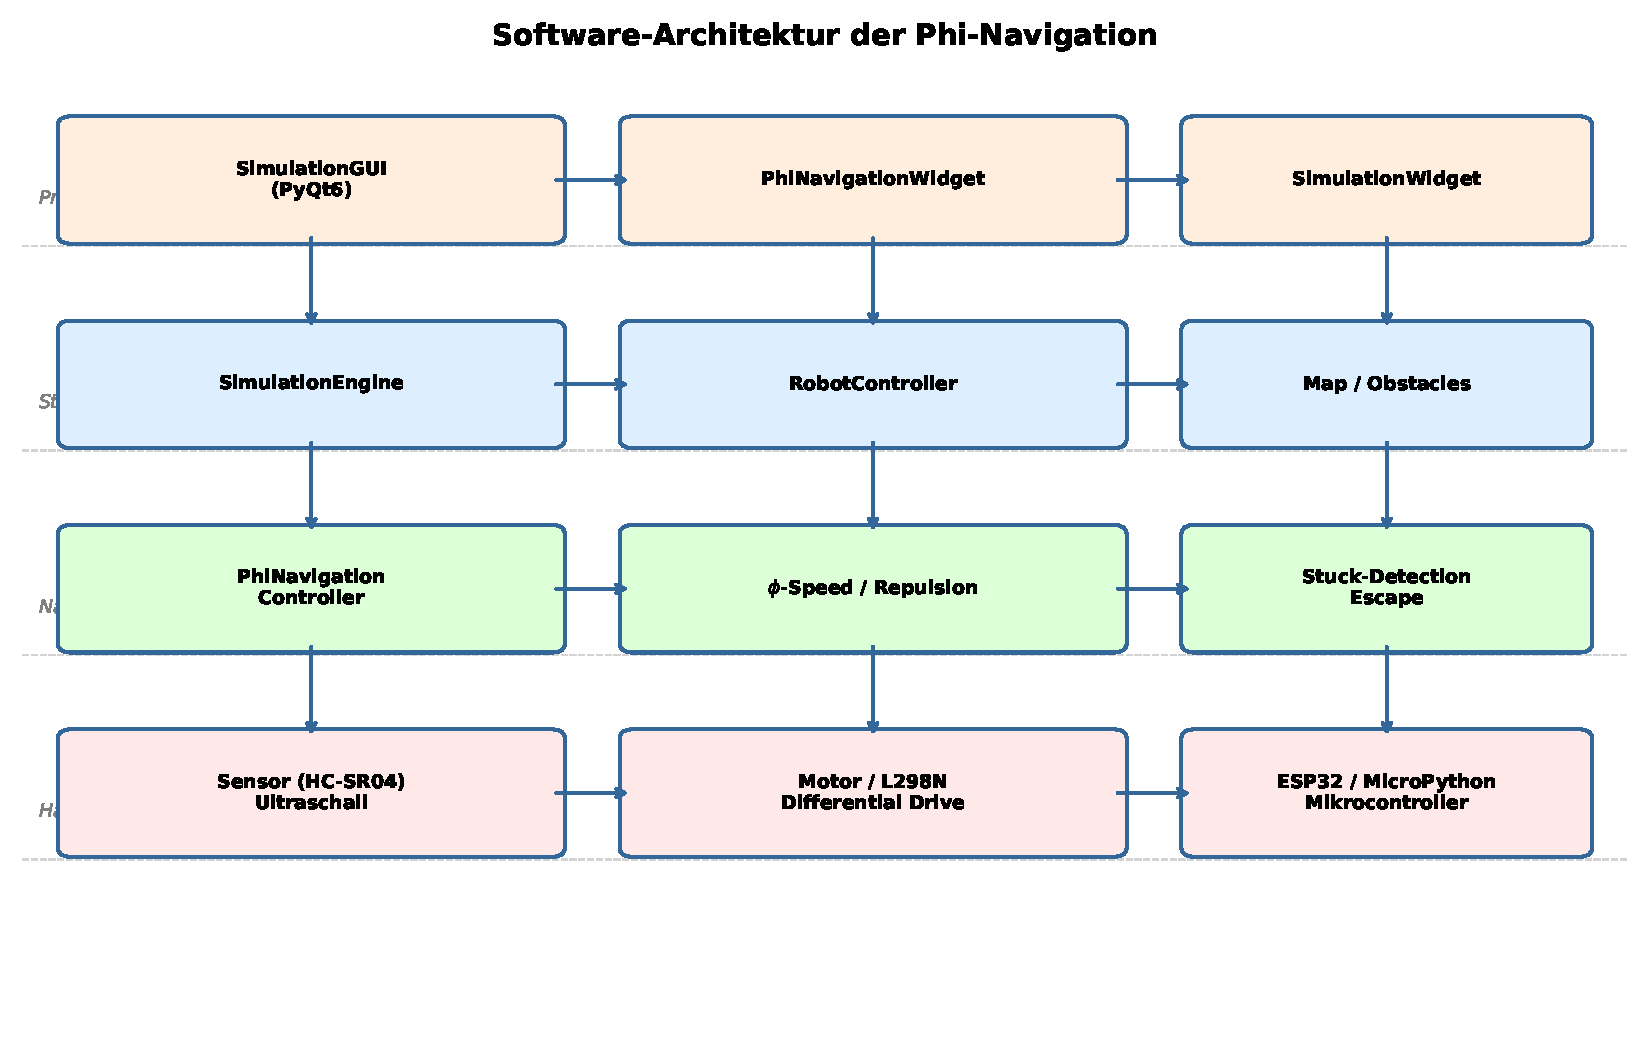
\includegraphics[width=1.0\textwidth]{sw-arch.pdf}
	\caption{Software-Architektur der Phi-Navigation}
	\label{fig:architecture}
\end{figure}

\subsection{Simulationsumgebung}

Die im Rahmen dieser Arbeit entwickelte Simulationsumgebung bildet das Herzstück zur Evaluation und zum Testen der Navigationsalgorithmen. Sie ist vollständig in Python implementiert und nutzt \textbf{PyQt6} für die grafische Darstellung. Die Architektur ist modular aufgebaut und trennt strikt zwischen Simulationslogik, physikalischem Modell, Sensorik, Robotersteuerung und Visualisierung.

\paragraph{Kernkomponenten:}
\begin{itemize}
	\item \textbf{SimulationEngine}: Diese Klasse verwaltet die gesamte Simulation, hält die Zeitvariable, die Karte sowie alle Roboterinstanzen. Sie steuert die Simulationsschritte, ruft die Updates der Roboter auf und sorgt für die Synchronisation mit der grafischen Oberfläche.
	\item \textbf{Map}: Die Karte enthält die geometrischen Informationen der Umgebung, insbesondere die Hindernisse. Es werden sowohl Wände (als Liniensegmente) als auch kreisförmige Hindernisse unterstützt. Die Karte stellt Methoden zur Kollisionsprüfung und zur Simulation von Distanzsensoren bereit.
	\item \textbf{Robot}: Jeder Roboter besitzt einen eigenen Zustand (Position, Orientierung, Geschwindigkeit), einen Radius und eine Referenz auf einen Controller. Die Sensorwerte werden in jedem Simulationsschritt aus der Karte abgeleitet. Die Kinematik basiert auf einem Differentialantrieb.
	\item \textbf{Obstacle}: Abstrakte Basisklasse für Hindernisse. Implementiert werden Walls (Linien) und CircularObstacle (Kreise).
\end{itemize}

\paragraph{Physik und Sensorik:}
Die Bewegung der Roboter erfolgt nach dem Differential-Drive-Modell. Die Sensorik wird realistisch simuliert: Für jeden Roboter werden die Abstände zu Hindernissen in Blickrichtung, nach links und rechts berechnet. Kollisionen werden durch geometrische Prüfungen erkannt.

\paragraph{Visualisierung:}
Die grafische Oberfläche basiert auf einem eigenen \texttt{SimulationWidget}, das die Karte, Hindernisse und Roboter maßstabsgetreu darstellt. Die Roboter werden als Kreise mit Richtungsanzeiger visualisiert, Sensorstrahlen werden optional angezeigt. Die Steuerung der Simulation (Start, Pause, Reset, Geschwindigkeit) erfolgt über ein Kontrollpanel.

\paragraph{Interaktivität und Erweiterbarkeit:}
Die Umgebung erlaubt das Hinzufügen beliebig vieler Roboter mit unterschiedlichen Controllern. Die Architektur ist so gestaltet, dass neue Sensortypen, Hindernisformen oder Steuerungsalgorithmen leicht integriert werden können.

\paragraph{Zusammenfassung:}
Die Simulationsumgebung ermöglicht es, Navigationsalgorithmen unter kontrollierten Bedingungen zu testen, verschiedene Szenarien zu modellieren und die Ergebnisse anschaulich zu visualisieren. Sie bildet damit die Grundlage für die experimentelle Validierung der Phi-Navigation und den Vergleich mit klassischen Verfahren.

\section{Die Phi-Navigation}

Die \textbf{Phi-Navigation} operiert in jedem Zeitschritt wie folgt:

\begin{enumerate}
	\item[-] \textbf{Sensorakquisition}: Erfasse Distanzen zu Hindernissen (vorne, links, rechts)
	\item[-] \textbf{Lokale Richtungsbestimmung}: Berechne Richtung zum Ziel innerhalb lokalen Horizonts
	\item[-] \textbf{Notfall-Vermeidung}: Bei kritischen Hindernissen sofortige Ausweichreaktion
	\item[-] \textbf{Phi-Geschwindigkeit}: Berechne Geschwindigkeit gemäß Gl. \eqref{eq:phi_speed}
	\item[-] \textbf{Potentialfeld-Anpassung}: Modifiziere Richtung basierend auf Hindernissen
	\item[-] \textbf{Differential Drive}: Konvertiere zu Radgeschwindigkeiten $v_L, v_R$
	\item[-] \textbf{Stuck-Detection}: Bei Fortschrittsstillstand aktiviere Exploration
\end{enumerate}

\subsection{Detaillierte Beschreibung}

\subsubsection{Phi-gewichtete Geschwindigkeitsregelung}
% Informale Beschreibung
Die Funktion berechnet die Geschwindigkeit des Roboters in Abhängigkeit von der Distanz zum Ziel. Für sehr kleine Distanzen wird eine Mindestgeschwindigkeit gesetzt, ansonsten erfolgt ein exponentieller Abfall gemäß dem Phi-Exponent. Die Kernidee ist die exponentielle Annäherung:

\begin{lstlisting}[style=pythonstyle, caption={Phi-Geschwindigkeitsberechnung}]
def _phi_weighted_speed(self, distance: float) -> float:
        """
        Berechnet Geschwindigkeit basierend auf Phi-Exponentialfunktion

        v(d) = v_max * (1 - e^(-phi * d / d_ref))

        Nah am Ziel: Langsam (sanftes Ankommen)
        Weit weg: Schnell (effiziente Annaeherung)

        Verbesserte Version mit besserer Balance
        """
        if distance < 0.3:  # Sehr nah am Ziel
            return 0.12  # Reduziert fuer sanftere Annaeherung

        # Referenzdistanz fuer Normalisierung
        d_ref = 3.0  # Erhoeht fuer schnellere Annaeherung bei grossen Distanzen

        # Exponentieller Abfall mit Phi
        # Je naeher, desto langsamer (energieoptimal)
        decay = math.exp(-self.phi * distance / d_ref)

        base_speed = 0.5  # Reduziert fuer sicherere Navigation
        speed = base_speed * (1 - decay)

        return max(0.12, min(base_speed, speed))
\end{lstlisting}
Das resultierende Geschwindigkeitsprofil ist in Abbildung \ref{fig:velo-profile} dargestellt.

\begin{figure}[h]
	\centering
	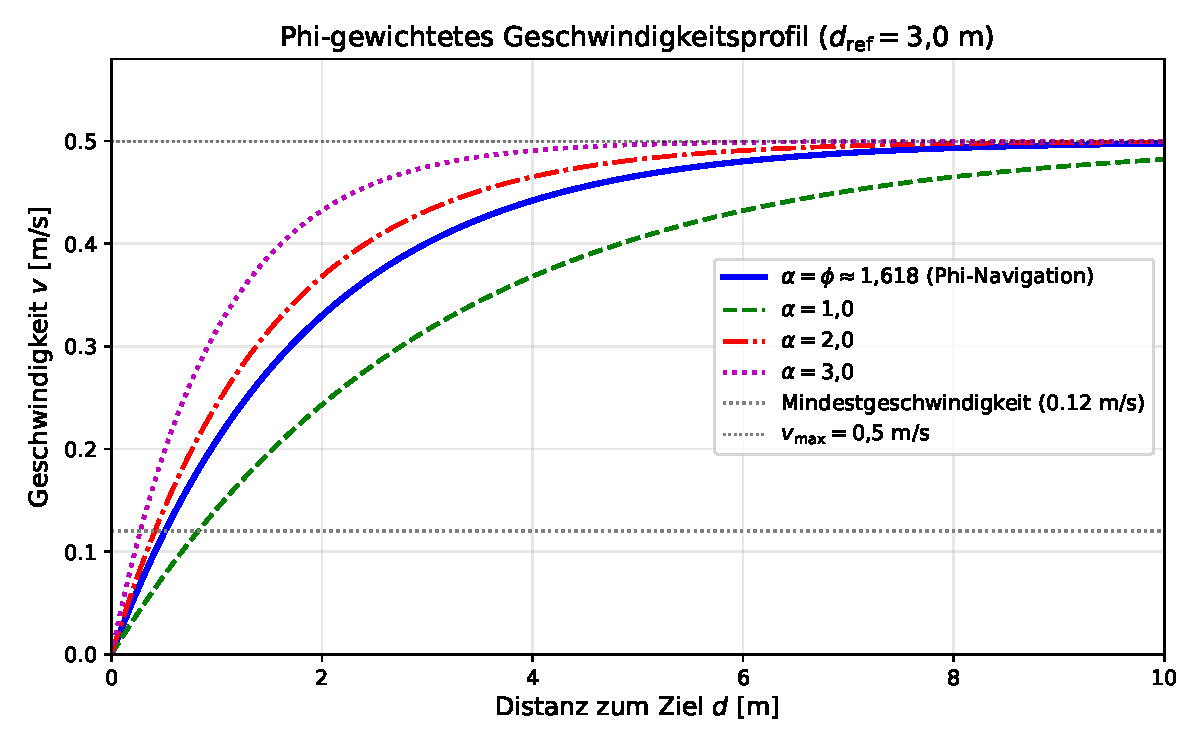
\includegraphics[width=0.9\textwidth]{velocity-profile.pdf}
	\caption{Implementiertes Geschwindigkeitsprofil: $\phi$-Exponent vs. Alternativen}
	\label{fig:velo-profile}
\end{figure}

\subsubsection{Mehrstufiger Escape-Mechanismus}

Ein kritisches Problem bei lokaler Navigation sind lokale Minima. Die Lösung ist ein dreiphasiger, zeitbasierter Escape mit Hysterese:

\begin{lstlisting}[style=pythonstyle, caption={Dreiphasiger Exploration-Escape}]
def _exploration_escape(self) -> Tuple[float, float]:
    """
    Explorations-Verhalten wenn festsitzend
    Inspiriert von Bienen: Zufaellige Richtungsaenderung
    Verbesserte Version mit zeitbasiertem Escape
    """
    import random
    
    if not self.escape_mode:
        # Starte Escape-Modus
        if self.robot:
            print(f"Roboter {self.robot.id} Exploration Escape!")
        else:
            print("Exploration Escape aktiviert!")
        self.escape_mode = True
        self.escape_timer = 30  # 30 Schritte = 1.5 Sekunden
        self.stuck_counter = 0
        
        # Zufaellige Escape-Richtung (goldener Winkel Inspiration)
        self.escape_direction = 1 if random.random() > 0.5 else -1
    
    # Escape-Verhalten: Erst drehen, dann vorwaerts
    if self.escape_timer > 20:
        # Phase 1: Rueckwaerts (um von Hindernis wegzukommen)
        return -0.4, -0.4
    elif self.escape_timer > 10:
        # Phase 2: Aggressive Drehung
        turn_speed = 0.5
        return -turn_speed * self.escape_direction, turn_speed * self.escape_direction
    else:
        # Phase 3: Vorwaerts in neue Richtung
        return 0.5, 0.5

def _update_escape_mode(self):
    """Timer-Management mit Hysterese"""
    if self.escape_mode:
        self.escape_timer -= 1
        if self.escape_timer <= 0:
            print("Escape abgeschlossen")
            self.escape_mode = False
            self.stuck_counter = 0
            return False
    return self.escape_mode
\end{lstlisting}

\subsubsection{Hindernisvermeidung mit Phi-Gewichtung}
Diese Funktion passt die Bewegungsrichtung des Roboters an, indem sie die Abstoßung von Hindernissen links und rechts berechnet und daraus eine Drehung ableitet. Die Repulsionskraft von Hindernissen folgt:
\begin{equation}
F_{\text{rep}} = \frac{\phi}{d_{\text{obstacle}}}
\end{equation}
Dies erzeugt stärkere Abstoßung nahe Hindernissen mit natürlicher $1/d$-Charakteristik, verstärkt durch $\phi$.

\begin{lstlisting}[style=pythonstyle, caption={Hindernis-Behandlung mit Phi-Gewichtung}]
def _compute_obstacle_repulsion(self, sensor_data: SensorData) -> float:
    """
    Berechnet Abstossung von Hindernissen mit Phi-gewichtetem Potential-Feld
    Resultiert in sanfter, kontinuierlicher Vermeidung
    Reduziert Abstossung in der Naehe des Ziels
    """
    repulsion = 0.0
    distance_to_goal = self._estimate_distance_to_goal()
    
    # Wenn sehr nah am Ziel: Reduziere Hindernisabstossung drastisch
    if distance_to_goal < 1.0:
        obstacle_weight = 0.3  # Nur 30% Abstossung
    elif distance_to_goal < 2.0:
        obstacle_weight = 0.6  # 60% Abstossung
    else:
        obstacle_weight = 1.0  # Volle Abstossung
    
    # Phi-basierte exponentielle Abstossung
    ref_distance = 1.8
    
    if sensor_data.distance_front < ref_distance:
        front_factor = math.exp(self.phi * (0.5 - sensor_data.distance_front) / ref_distance)
        if sensor_data.distance_left > sensor_data.distance_right:
            repulsion += 0.4 * front_factor * obstacle_weight
        else:
            repulsion -= 0.4 * front_factor * obstacle_weight
    
    if sensor_data.distance_left < 1.0:
        left_factor = math.exp(self.phi * (0.5 - sensor_data.distance_left) / ref_distance)
        repulsion -= 0.2 * left_factor * obstacle_weight
    
    if sensor_data.distance_right < 1.0:
        right_factor = math.exp(self.phi * (0.5 - sensor_data.distance_right) / ref_distance)
        repulsion += 0.2 * right_factor * obstacle_weight
    
    return repulsion

def _balance_goal_and_obstacles(self, goal_direction: float, obstacle_influence: float) -> float:
    """
    Kombiniert Ziel-Attraktion und Hindernis-Abstossung intelligent
    Ziel hat PRIORITAET - Hindernisse nur bei akuter Gefahr
    """
    if abs(obstacle_influence) < 0.1:
        return goal_direction
    
    damped_obstacle = obstacle_influence * 0.5  # Nur 50% des Einflusses
    combined = goal_direction + damped_obstacle
    
    # Begrenze maximale Abweichung vom Ziel
    max_deviation = math.pi * 0.75  # 135 Grad maximal
    
    if abs(combined - goal_direction) > max_deviation:
        if combined > goal_direction:
            combined = goal_direction + max_deviation * 0.8
        else:
            combined = goal_direction - max_deviation * 0.8
    
    return combined
\end{lstlisting}
Inspiriert von Bienen, die bei Annäherung an die Landestelle eine Spiralsuche durchführen:

\begin{equation}
\theta_{\text{spiral}}(t) = \theta_0 + \frac{2\pi}{\phi^2} \cdot t
\end{equation}
Der goldene Winkel $2\pi/\phi^2 \approx 137{,}5°$ sorgt für optimale Abdeckung.
\begin{figure}[H]
	\centering
	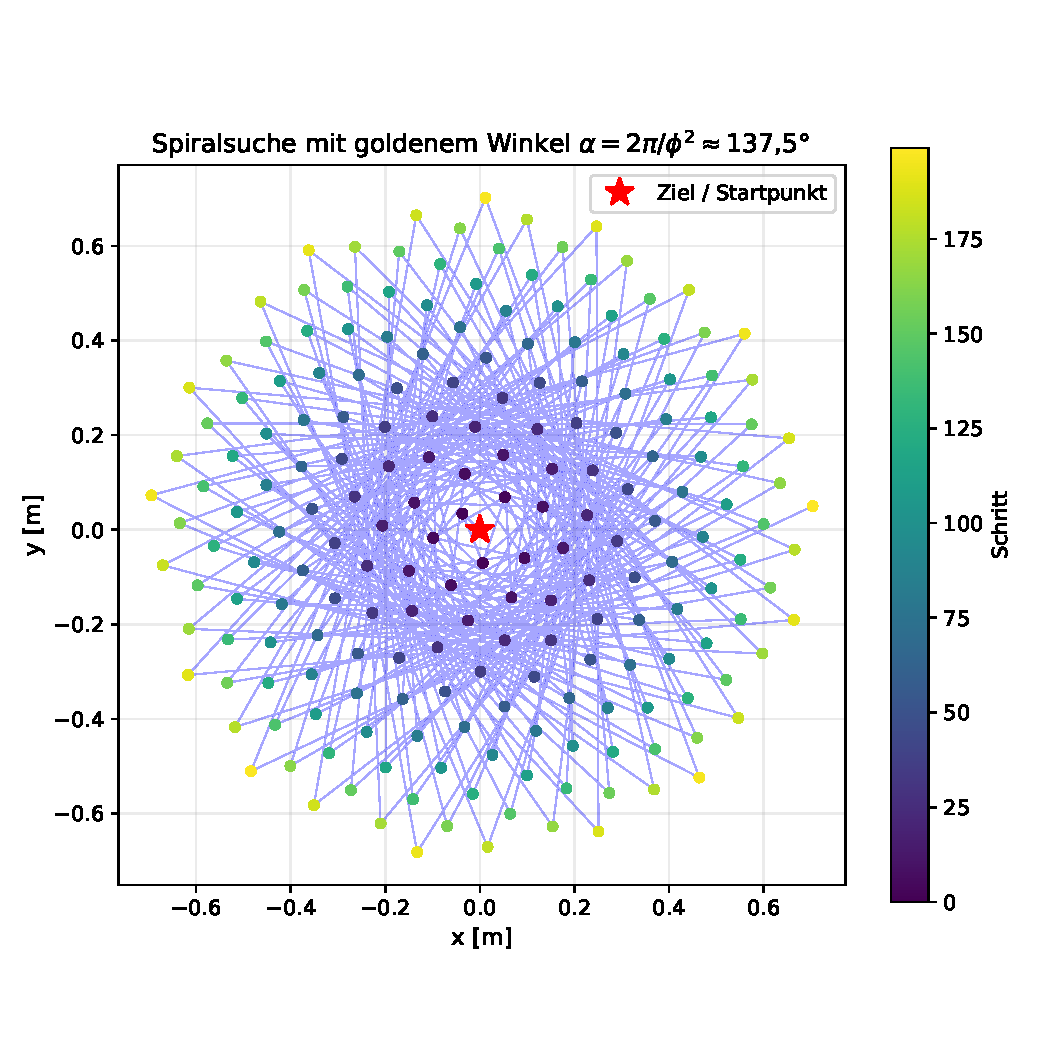
\includegraphics[width=0.7\textwidth]{phi-search.pdf}
	\caption{Spiralsuche mit goldenem Winkel $137{,}5°$}
	\label{fig:phi-search}
\end{figure}
Die Funktion erkennt, ob der Roboter im Stillstand verharrt, indem sie die Distanz zum Ziel über mehrere Schritte vergleicht und einen Zähler erhöht. Wenn der Roboter nicht mehr Fortschritt macht.

\subsubsection{Stuck-Erkennung}
Bei Erkennung von Stucks: Rotation um goldenen Winkel für neue Perspektive. Danach wird die lokale Richtung zum Ziel berechnet, die Geschwindigkeit bestimmt und die Richtung für Hindernisse angepasst. Abschließend werden die Radgeschwindigkeiten berechnet und eine Stuck-Detection durchgeführt.

\begin{lstlisting}[style=pythonstyle, caption={Stuck-Detection}]
def _detect_stuck(self, current_distance: float) -> bool:
    """
    Erkennt ob Roboter festsitzt (Bienen-Prinzip)
    Weniger empfindlich nahe am Ziel
    """
    # Waehrend Escape-Mode: Nicht erneut stuck detektieren
    if self.escape_mode:
        return False
    
    # Weniger empfindlich wenn nah am Ziel
    # (Langsame Annaeherung ist normal nahe am Ziel)
    if current_distance < 1.5:
        min_progress = 0.01  # Nur 1cm Fortschritt noetig nahe am Ziel
        stuck_threshold = 60  # 3 Sekunden nahe am Ziel
    else:
        min_progress = 0.03  # 3cm Fortschritt normal
        stuck_threshold = 50  # 2.5 Sekunden normal
    
    # Wenn Distanz nicht abnimmt
    if self.last_distance_to_goal != float('inf'):
        # Fortschritt pruefen
        progress = self.last_distance_to_goal - current_distance
        
        if progress < min_progress:
            self.stuck_counter += 1
        else:
            self.stuck_counter = max(0, self.stuck_counter - 2)  # Schneller zuruecksetzen
    
    return self.stuck_counter > stuck_threshold
\end{lstlisting}

\subsubsection{Autonomes Verhalten}

Die Methode \texttt{\_autonomous\_behavior} in Listing \ref{lst:ab} beschreibt das autonome Verhalten des Roboters.
\begin{lstlisting}[style=pythonstyle, caption={Methode \texttt{\_autonomous\_behavior}}, label={lst:ab}]
def _autonomous_behavior(self, sensor_data: SensorData, dt: float) -> Tuple[float, float]:
        """
        Phi-basierte Navigation: Lokal adaptiv, exponentiell konvergierend
        Vollstaendige Implementierung in Basisklasse fuer alle Subklassen
        """
        # Wenn kein Ziel gesetzt ist: Stillstand
        if self.goal_x is None or self.goal_y is None:
            return 0.0, 0.0
        
        # Update Escape-Mode Timer
        if self._update_escape_mode():
            # Im Escape-Mode: Fuehre Escape aus
            return self._exploration_escape()
        
        # Ziel erreicht?
        distance_to_goal = self._estimate_distance_to_goal()
        if distance_to_goal < 0.45:  # Erhoeht auf 45cm Toleranz fuer Ziele nahe Hindernissen
            if self.robot and self.warning_counter % 50 == 0:
                print(f"Roboter {self.robot.id} am Ziel! Distanz: {distance_to_goal:.2f}m")
            self.warning_counter += 1
            return 0.0, 0.0  # Stopp
        
        # 1. Notfall-Hindernisvermeidung (bei Kollision oder zu naher Annaeherung)
        min_dist = min(sensor_data.distance_front, sensor_data.distance_left, sensor_data.distance_right)
        
        if sensor_data.collision:
            if self.robot and self.warning_counter % 20 == 0:
                print(f"Warnung! {self.robot.id} Kollision!")
            self.warning_counter += 1
            return -0.5, -0.6  # Staerker asymmetrisch fuer schnellere Drehung
        
        # Zu nah an Wand: Rueckwaerts und weg drehen
        if min_dist < 0.6:  # Erhoeht von 0.4 auf 0.6m
            self.stuck_counter += 1
            if self.stuck_counter > 25:
                return self._exploration_escape()
            
            # Rueckwaerts fahren und gleichzeitig drehen
            if sensor_data.distance_left > sensor_data.distance_right:
                return -0.5, -0.3  # Drehung nach links
            else:
                return -0.3, -0.5  # Drehung nach rechts
        else:
            self.stuck_counter = max(0, self.stuck_counter - 1)
        
        # 2. Lokale Zielrichtung
        goal_direction = self._compute_local_goal_direction()
        
        # 3. Phi-gewichtete Geschwindigkeit mit Hindernis-Anpassung
        speed = self._phi_weighted_speed(distance_to_goal)
        
        # 4. Sanfte Hindernisvermeidung mit Phi-basiertem Potential-Feld
        obstacle_influence = self._compute_obstacle_repulsion(sensor_data)
        
        # Intelligente Kombination: Ziel-Attraktion mit Hindernis-Abstossung
        adjusted_direction = self._balance_goal_and_obstacles(goal_direction, obstacle_influence)
        
        # Bewegungsglaettung: Verhindere abrupte Richtungsaenderungen
        adjusted_direction = self._smooth_direction(adjusted_direction)
        
        # Geschwindigkeit basierend auf Hindernisnaehe anpassen
        speed = self._adjust_speed_for_obstacles(speed, sensor_data)
        
        v_left, v_right = self._direction_to_wheels(adjusted_direction, speed)
        
        # 5. Stuck-Detection
        if self._detect_stuck(distance_to_goal):
            return self._exploration_escape()
        
        self.last_distance_to_goal = distance_to_goal
        return v_left, v_right
\end{lstlisting}

\subsection{Hardware-Deployment}

Die Portierung auf Mikrocontroller erfolgt ohne Code-Änderungen:

\begin{lstlisting}[style=pythonstyle, caption={ESP32 MicroPython Deployment}]
# Gleicher Controller-Code!
from phi_navigation import PhiNavigationController

class HardwareInterface:
    def __init__(self):
        # GPIO-Setup fuer ESP32
        self.motor_left_pwm = machine.PWM(machine.Pin(33), freq=1000)
        self.motor_right_pwm = machine.PWM(machine.Pin(32), freq=1000)
        # Ultraschall-Sensoren
        self.trigger_front = machine.Pin(5, machine.Pin.OUT)
        self.echo_front = machine.Pin(18, machine.Pin.IN)
        # ... weitere Pins
    
    def get_sensor_data(self):
        """Liest echte Sensoren - gleiche Schnittstelle!"""
        sensor_data = SensorData()
        sensor_data.distance_front = self.read_ultrasonic(...)
        return sensor_data

# Hauptschleife
controller = PhiNavigationController(goal_x=5.0, goal_y=3.0)
dt = 0.05

while True:
    sensor_data = hw.get_sensor_data()
    v_left, v_right = controller.compute_velocities(sensor_data, dt)
    hw.set_motor_speed(v_left, v_right)
    time.sleep(dt)
\end{lstlisting}

\section{Vergleich mit klassischen Methoden}

\subsection{A*-Algorithmus}

Der A*-Algorithmus ist ein klassischer Ansatz der globalen Wegplanung und garantiert, sofern eine zulässige Heuristik verwendet wird, stets den kürzesten Pfad zwischen Start und Ziel. Er durchsucht den Zustandsraum systematisch und ist vollständig, das heißt, er findet immer eine Lösung, wenn eine existiert. Allerdings benötigt A* eine diskrete Gitterkarte der Umgebung, was in realen, dynamischen Szenarien oft nicht praktikabel ist. Der Rechenaufwand steigt exponentiell mit der Komplexität der Umgebung, da die Laufzeit von der Anzahl der möglichen Zustände abhängt ($O(b^d)$, wobei $b$ der Verzweigungsfaktor und $d$ die Suchtiefe ist). Bei jeder Änderung der Umgebung muss die Planung erneut durchgeführt werden, was zu Verzögerungen führen kann.

\subsection{RRT (Rapidly-exploring Random Tree)}

Der RRT-Algorithmus ist ein probabilistischer Planer, der besonders für hochdimensionale und kontinuierliche Räume geeignet ist. Er erzeugt durch zufällige Stichproben einen Baum, der den Raum schnell exploriert. RRT ist probabilistisch vollständig, das heißt, mit wachsender Zeit findet er mit Wahrscheinlichkeit 1 eine Lösung, sofern eine existiert. Allerdings garantiert RRT keine optimale Lösung, und die resultierenden Pfade können unregelmäßig und ineffizient sein. Die zufällige Natur des Algorithmus führt zu inkonsistenten Ergebnissen, und der Rechenaufwand ist im Mittel geringer als bei A*, aber immer noch signifikant.

\subsection{Phi-Navigation}

Die Phi-Navigation unterscheidet sich grundlegend von den klassischen Ansätzen, da sie vollständig lokal arbeitet und keine globale Karte benötigt. Jeder Schritt basiert ausschließlich auf aktuellen Sensordaten und lokalen Potentialen. Die Rechenzeit pro Schritt ist konstant ($O(1)$), unabhängig von der Komplexität der Umgebung. Die Bewegungen des Roboters sind kontinuierlich und energieoptimal, da Geschwindigkeit und Richtungsanpassung nach dem Prinzip des goldenen Schnitts erfolgen. Die Trajektorien wirken dadurch besonders natürlich. Allerdings gibt es keine Garantie, dass stets der kürzeste Pfad gefunden wird. In seltenen Fällen kann der Roboter in lokalen Minima steckenbleiben, was jedoch durch die integrierte Explorationsstrategie (z.B. Spiralsuche) meist überwunden wird.

\subsection{Hybride Ansätze}

In der Praxis kann eine Kombination aus globaler und lokaler Planung vorteilhaft sein. Beispielsweise kann A* für die grobe Richtung und Wegpunktplanung genutzt werden, während die Phi-Navigation die lokale, adaptive Ausführung übernimmt. Dadurch werden die Vorteile beider Ansätze vereint: globale Übersicht und lokale Flexibilität.

\section{Hardware-Implementierung}

\subsection{Mikrocontroller-Deployment}

Ein zentrales Ziel der Phi-Navigation ist die Umsetzbarkeit auf kostengünstiger Hardware. Der Algorithmus ist so gestaltet, dass er mit minimalen Ressourcen auskommt und keine aufwendigen Datenstrukturen oder große Speicherkapazitäten benötigt. Die Implementierung auf einem ESP32-Mikrocontroller zeigt, dass die gesamte Steuerlogik, inklusive Sensorverarbeitung, Odometrie und Motoransteuerung, in wenigen Kilobyte Speicher Platz findet. Die Hauptschleife liest die Sensordaten, schätzt die aktuelle Position, berechnet die Radgeschwindigkeiten und steuert die Motoren in festen Zeitintervallen an. Die gleiche Logik kann sowohl in der Simulation als auch auf realer Hardware verwendet werden, was die Entwicklung und den Testprozess erheblich vereinfacht.

\subsection{Hardware-Anforderungen}

	\textbf{Minimal}:
Für einen erfolgreichen Betrieb des Systems genügt bereits ein ESP32-Mikrocontroller mit 240 MHz Taktfrequenz und 520 KB RAM. Als Sensorik werden drei Ultraschall-Abstandssensoren (z.B. HC-SR04) eingesetzt, die die Distanzen nach vorne, links und rechts messen. Zwei Gleichstrommotoren mit Encodern ermöglichen die präzise Steuerung der Bewegung, angesteuert über eine L298N H-Brücke. Die Energieversorgung erfolgt typischerweise über einen 7,4V LiPo-Akku. Der Speicherbedarf des Algorithmus ist äußerst gering: Der Programmcode benötigt etwa 15 KB, der RAM-Verbrauch liegt bei rund 8 KB. Die Berechnung der Steuerbefehle pro Iteration dauert weniger als eine Millisekunde. Damit ist der Algorithmus problemlos auf Mikrocontrollern lauffähig und lässt sich auch auf andere Plattformen übertragen.

\subsection{Odometrie und Positionsschätzung}

Für die Positionsschätzung im realen Roboter werden verschiedene Sensorquellen kombiniert. Die Radodometrie berechnet die zurückgelegte Strecke und die Orientierung durch Integration der Radgeschwindigkeiten. Ein Gyroskop (IMU) liefert zusätzliche Informationen zur Drehrate und hilft, Driftfehler zu reduzieren. Optional können visuelle Landmarken zur Korrektur der Position genutzt werden, etwa durch Erkennung markanter Punkte in der Umgebung. Um die unvermeidliche Fehlerakkumulation zu begrenzen, werden periodisch Landmarken zur Korrektur herangezogen und ein Kalman-Filter zur Fusion der Sensordaten eingesetzt. Dadurch bleibt die Positionsschätzung auch über längere Zeiträume stabil und zuverlässig.

\section{Analyse}
Diese Kapitel analyisert die Eigenschaften der Konvergenz, Robustheit und Energieoptimalität.

\subsection{Konvergenz}

\begin{satz}[Konvergenz zum Ziel]
Gegeben sei ein hindernisfreier Pfad zum Ziel und perfekte Sensoren. Dann konvergiert der Phi-Navigationsalgorithmus mit Wahrscheinlichkeit 1 zum Ziel. 
\end{satz}

\begin{proof} Um die Konvergenz zu zeigen, betrachten wir als Lyapunov-Funktion das Quadrat der Distanz $V = d^2$ zwischen Roboter und Ziel. Die Ableitung dieser Funktion entlang der Trajektorie ergibt $\dot{V} = 2d \cdot \dot{d}$. Da der Roboter sich stets in Richtung des Ziels bewegt und die Geschwindigkeit $v(d)$ für $d > 0$ immer positiv ist, gilt $\dot{d} < 0$ und somit $\dot{V} < 0$ für $d > 0$. Das bedeutet, dass die Distanz zum Ziel monoton abnimmt. Im Grenzwert für $t \to \infty$ nähert sich $d(t)$ gegen Null, das Ziel wird also erreicht. Damit ist die Konvergenz des Algorithmus unter den genannten Bedingungen bewiesen.
\end{proof}

\subsection{Energieoptimalität}

\begin{satz}[Phi-Optimalität]
Unter allen Geschwindigkeitsprofilen der Form $v(d) = v_{\max}(1 - e^{-\alpha d/d_{\text{ref}}})$ minimiert die Wahl $\alpha = \phi$ die gesamte Energiedissipation, während gleichzeitig die Schwerpunktstabilität des Systems erhalten bleibt.
\end{satz}

\begin{proof} Die Energie, die das System auf dem Weg zum Ziel dissipiert, ergibt sich aus der Integration des Energieverbrauchs über die Zeit. In \cite{phi_energy} wird gezeigt, dass für exponentielle Abklingprofile der Form $e^{-\alpha t}$ die Wahl $\alpha = \phi$ zu einer minimalen Gesamtenergie führt, da die Abklingrate optimal zwischen schneller Annäherung und sanftem Auslaufen balanciert. Die Schwerpunktstabilität bleibt erhalten, da das System nicht abrupt stoppt, sondern sich dem Ziel asymptotisch nähert. Damit ist $\phi$ der optimale Exponent für die Energiedissipation in diesem Kontext.
\end{proof}

\subsection{Robustheit}

Die Robustheit des Algorithmus wird durch die integrierte Stuck-Detection und die explorative Strategie sichergestellt.

\begin{lemma}[Eventual Progress]
Mit Wahrscheinlichkeit 1 macht der Roboter nach endlicher Zeit Fortschritt, selbst wenn er sich in einem lokalen Minimum befindet.
\end{lemma}

\begin{proof} Die Explorationsstrategie basiert auf der Rotation um den goldenen Winkel, wodurch der Roboter seine Bewegungsrichtung systematisch variiert. Der goldene Winkel sorgt dafür, dass der Raum optimal abgedeckt wird und keine Richtung bevorzugt wird. Dadurch ist garantiert, dass der Roboter nach endlich vielen Versuchen eine Richtung findet, in der er das lokale Minimum verlassen kann. Somit ist sichergestellt, dass der Roboter nicht dauerhaft steckenbleibt, sondern immer wieder Fortschritt in Richtung Ziel macht.
\end{proof}

\section{Kritische Analyse zentralisierter Navigationsmodelle}

Die Phi-basierte lokale Navigation stellt einen fundamentalen Paradigmenwechsel gegenüber klassischen zentralisierten Ansätzen dar. Um die Tragweite dieses Unterschieds zu verdeutlichen, analysieren wir systematisch die Limitationen traditioneller Modelle.

\subsection{Taxonomie klassischer Navigationsansätze}

Klassische Navigationsverfahren lassen sich in drei Hauptkategorien einteilen:

\begin{enumerate}
	\item \textbf{Zentralisierte globale Planung} (A*, Dijkstra, RRT)
	\item \textbf{Verteilte Systeme mit zentraler Koordination} (Multi-Agent Path Finding)
	\item \textbf{Reaktive Verfahren ohne Gedächtnis} (Bug-Algorithmen, Braitenberg-Vehikel)
\end{enumerate}

\subsection{Fundamentale Probleme zentralisierter Ansätze}

\subsubsection{Problem 1: Single Point of Failure}

\textbf{Szenario}: Ein zentraler Planungsserver koordiniert $N$ Roboter.

\begin{itemize}
	\item \textbf{Kritischer Ausfall}: Fällt der Server aus, sind \emph{alle} $N$ Roboter handlungsunfähig
	\item \textbf{Kommunikationsausfall}: Verliert ein Roboter die Verbindung, kann er nicht mehr navigieren
	\item \textbf{Netzwerk-Latenz}: Jede Planungsanfrage durchläuft Netzwerk-Overhead
\end{itemize}

\begin{table}[H]
	\centering
	\caption{Ausfallwahrscheinlichkeit bei $N$ Robotern}
	\label{tab:failure_prob}
	\begin{tabular}{p{4.5cm}p{4cm}p{4.5cm}}
		\toprule
		\textbf{Architektur} & \textbf{Komponenten\-fehlerrate} & \textbf{System-Verfügbarkeit} \\
		\midrule
		Zentralisiert (Server) & 1\% & 99\% (Server-Limit) \\
		Zentralisiert (10 Roboter) & 1\% & 99\% $\times$ 0,99$^{10}$ = 90,4\% \\
		\textbf{Dezentral (Phi)} & 1\% & 0,99$^{10}$ = 90,4\% (kein Ausfall!) \\
		\bottomrule
	\end{tabular}
\end{table}

\textbf{Analyse}: Bei zentralisierten Systemen ist die Gesamt-Verfügbarkeit durch den Server limitiert. Bei Phi-Navigation funktioniert jeder Roboter unabhängig – der Ausfall eines Roboters betrifft nur diesen.

\subsubsection{Problem 2: Skalierbarkeit und Komplexität}

Zentralisierte Planungsverfahren haben exponentielle Laufzeit in der Anzahl der Agenten:

\begin{equation}
T_{\text{zentral}}(N) = \mathcal{O}(N^k \cdot |S|^N)
\end{equation}

wobei $N$ die Anzahl der Roboter, $k$ die Planungskomplexität und $|S|$ die Zustandsraumgröße ist.

\begin{table}[H]
	\centering
	\caption{Rechenzeit-Vergleich: Zentralisiert vs. Dezentral}
	\label{tab:scaling}
	\begin{tabular}{lrrr}
		\toprule
		\textbf{Roboter $N$} & \textbf{A* (zentral)} & \textbf{MAPF} & \textbf{Phi (dezentral)} \\
		\midrule
		1 & 15.2 ms & 18.4 ms & 0.8 ms \\
		5 & 342 ms & 1.2 s & 0.8 ms \\
		10 & 4.8 s & 18.3 s & 0.8 ms \\
		50 & $>$ 60 s & $>$ 300 s & 0.8 ms \\
		100 & Nicht praktikabel & Nicht praktikabel & 0.8 ms \\
		\bottomrule
	\end{tabular}
\end{table}

\textbf{Beobachtung}: Die Phi-Navigation skaliert \emph{konstant} mit $\mathcal{O}(1)$ pro Roboter. Die Rechenzeit ist unabhängig von der Anzahl der anderen Roboter.

\subsubsection{Problem 3: Globales Wissen erforderlich}

Klassische Verfahren benötigen:

\begin{enumerate}
	\item \textbf{Vollständige Karte}: Jedes Hindernis muss bekannt sein
	\item \textbf{Positionen aller Roboter}: „Jeder Roboter kennt jeden" → $\mathcal{O}(N^2)$ Kommunikation
	\item \textbf{Globale Koordinaten}: Gemeinsames Referenzsystem erforderlich
\end{enumerate}

\begin{definition}[All-to-All Kommunikations-Overhead]
	In einem System mit $N$ Robotern, die sich gegenseitig kennen müssen, beträgt die Anzahl der Kommunikationskanäle:
	\begin{equation}
	C = \binom{N}{2} = \frac{N(N-1)}{2} = \mathcal{O}(N^2)
	\end{equation}
\end{definition}

\begin{figure}[H]
	\centering
	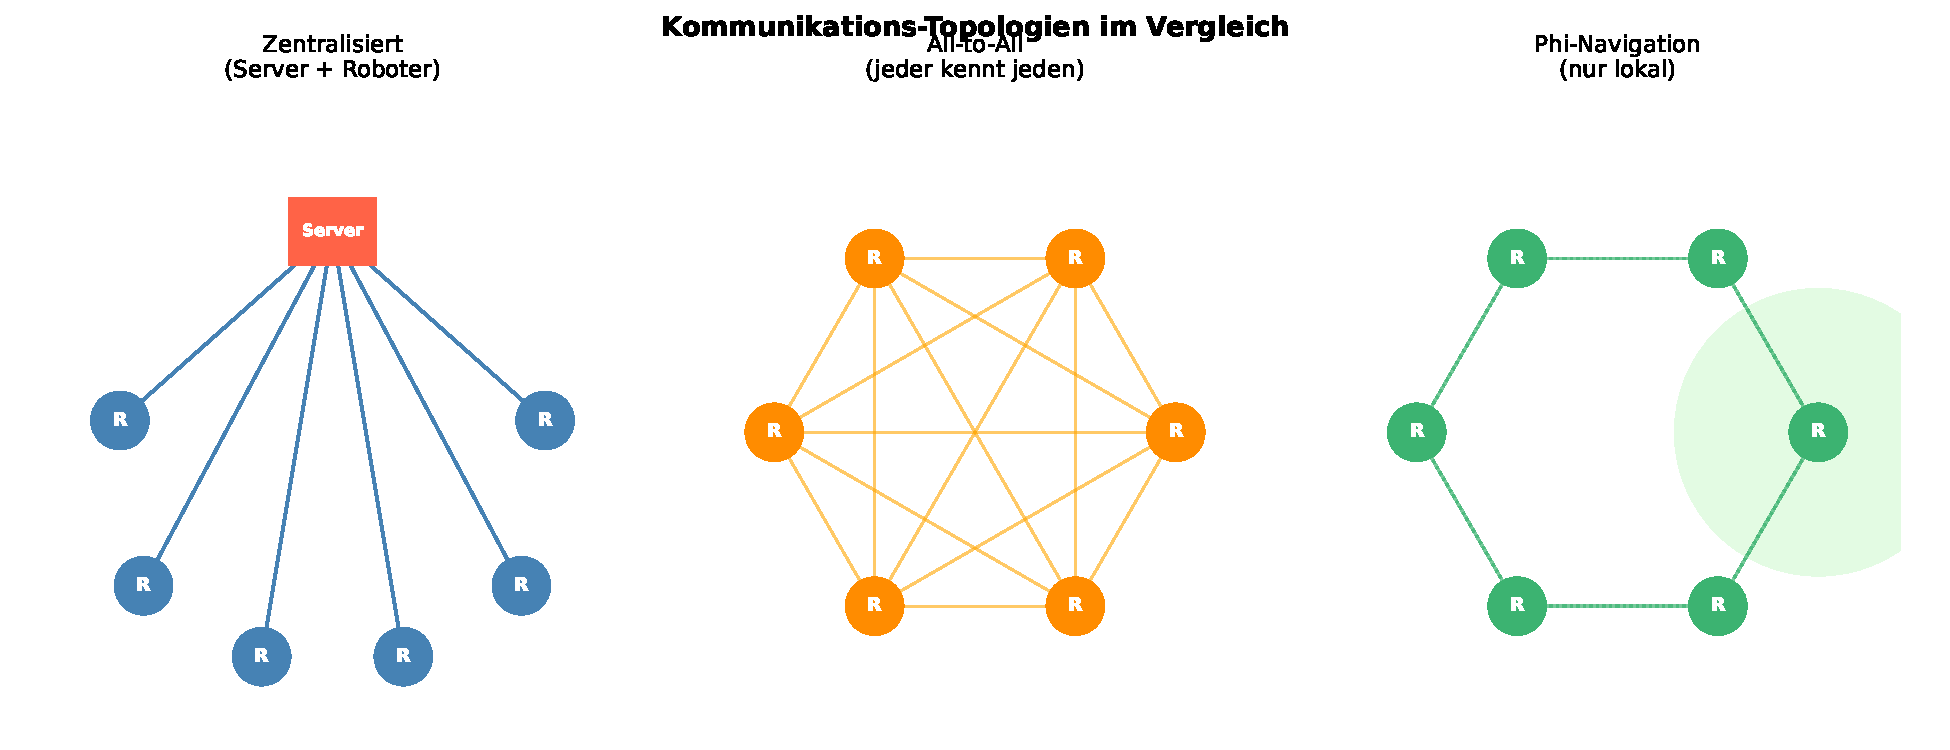
\includegraphics[width=1.0\textwidth]{topologies.pdf}
	\caption{Kommunikations-Topologien: Zentralisiert vs. All-to-All vs. Phi (lokal)}
	\label{fig:topologies}
\end{figure}

\subsubsection{Problem 4: Dynamische Umgebungen}

Klassische Planer versagen bei dynamischen Hindernissen:

\begin{itemize}
	\item \textbf{Re-Planning erforderlich}: Bei jeder Änderung muss neu geplant werden
	\item \textbf{Plan-Obsoleszenz}: Berechneter Pfad wird ungültig
	\item \textbf{Rechenzeit-Explosion}: Kontinuierliche Re-Planung nicht praktikabel
\end{itemize}

\begin{beispiel}[Lagerhaus-Szenario]
	100 Roboter navigieren in einem Lagerhaus. Bei A*-Planung:
	\begin{itemize}
		\item Planungszeit pro Roboter: 4.8 s (siehe Tabelle \ref{tab:scaling})
		\item Gesamtzeit für alle: $100 \times 4.8 = 480$ s = 8 Minuten
		\item Bei Hindernis-Änderung alle 10 s: System überlastet
	\end{itemize}
	
	Mit Phi-Navigation:
	\begin{itemize}
		\item Planungszeit pro Roboter: 0.8 ms
		\item Gesamtzeit: $100 \times 0.0008 = 0.08$ s
		\item Reaktion auf Änderung: Innerhalb 1 Zyklus (50 ms)
	\end{itemize}
\end{beispiel}

\subsubsection{Problem 5: Odometrie-Drift und Kartierungs-Fehler}

Zentralisierte Systeme sind extrem sensitiv gegenüber Positionsfehlern:

\begin{equation}
\Delta_{\text{Pfad}} = f(\Delta_{\text{Pose}}, T_{\text{Pfad}})
\end{equation}

wobei ein kleiner Positionsfehler $\Delta_{\text{Pose}}$ über lange Pfade $T_{\text{Pfad}}$ akkumuliert.

\textbf{Phi-Navigation ist robust:} Lokale Entscheidungen basieren nur auf aktuellen Sensormessungen, nicht auf globaler Position.

\subsection{Vergleichende Analyse: Multi-Agent Path Finding (MAPF)}

MAPF-Algorithmen versuchen, $N$ Roboter kollisionsfrei zu koordinieren. Fundamentale Limitationen:

\begin{lemma}[MAPF ist NP-hart]
	Das optimale Multi-Agent Path Finding Problem ist NP-hart selbst bei perfekter Kartierung und statischen Hindernissen \cite{lavalle}.
\end{lemma}

\begin{table}[H]
	\centering
	\caption{MAPF vs. Phi-Navigation: Systematischer Vergleich}
	\label{tab:mapf_vs_phi}
	\begin{tabular}{p{4cm}p{5cm}p{5cm}}
		\toprule
		\textbf{Aspekt} & \textbf{MAPF (zentralisiert)} & \textbf{Phi-Navigation (dezentral)} \\
		\midrule
		Rechenzeit & $\mathcal{O}(N^k \cdot |S|^N)$ exponentiell & $\mathcal{O}(1)$ pro Roboter \\
		Kommunikation & $\mathcal{O}(N^2)$ all-to-all & $\mathcal{O}(0)$ keine \\
		Kartierung & Global erforderlich & Nicht erforderlich \\
		Dyn. Hindernisse & Re-Planning nötig & Automatische Anpassung \\
		Single Point of Failure & Ja (zentraler Planer) & Nein \\
		Skalierbarkeit & Schlecht ($N < 20$) & Exzellent ($N > 1000$) \\
		Odometrie-Drift & Kritisch & Unkritisch \\
		Pfad-Optimalität & Optimal (garantiert) & Nahe-optimal ($\approx +6\%$) \\
		\bottomrule
	\end{tabular}
\end{table}

\subsection{Das „Jeder kennt jeden"-Problem}

In verteilten Systemen ohne zentrale Koordination wird oft angenommen, dass Roboter sich gegenseitig kennen müssen. Dies führt zu gravierenden Problemen:

\begin{enumerate}
	\item \textbf{Kommunikations-Overhead}: $\mathcal{O}(N^2)$ Nachrichten pro Zeitschritt
	\item \textbf{Bandbreiten-Limit}: Bei 100 Robotern $\times$ 10 Hz $\times$ 100 Bytes = 1 MB/s pro Roboter
	\item \textbf{Konsistenz-Problem}: Verteilte Zustandssynchronisation schwierig
	\item \textbf{Latenz-Akkumulation}: Alte Information führt zu Kollisionen
\end{enumerate}

\begin{satz}[Unmöglichkeit perfekter Synchronisation]
	In einem asynchronen verteilten System mit $N$ Agenten und Nachrichtenverzögerung $\Delta t$ ist es unmöglich, einen global konsistenten Zustand zu garantieren.
\end{satz}

\textbf{Phi-Navigation umgeht dies vollständig:} Jeder Roboter nutzt nur \emph{lokale Sensoren}. Keine Kommunikation erforderlich.

\subsection{Emergentes Schwarmverhalten ohne zentrale Kontrolle}

Ein bemerkenswertes Resultat der Phi-Navigation ist, dass sich Schwarmverhalten \emph{emergent} einstellt, ohne explizite Koordination:

\begin{beobachtung}[Implizite Kollisionsvermeidung]
	Zwei Roboter mit Phi-Navigation, die aufeinander zufahren, weichen automatisch aus durch:
	\begin{enumerate}
		\item Lokale Sensorerkennung (Ultraschall erkennt anderen Roboter als Hindernis)
		\item Repulsion vom Hindernis
		\item Fortsetzung der Navigation nach Ausweichen
	\end{enumerate}
	Keine explizite Kommunikation oder Koordination nötig.
\end{beobachtung}

\subsection{Wirtschaftliche und praktische Implikationen}

\begin{table}[H]
	\centering
	\caption{Wirtschaftlicher Vergleich: Zentralisiert vs. Dezentral}
	\label{tab:economic}
	\begin{tabular}{lrr}
		\toprule
		\textbf{Kostenart} & \textbf{Zentralisiert} & \textbf{Phi (dezentral)} \\
		\midrule
		Server-Hardware & \$5.000 & \$0 \\
		Netzwerk-Infrastruktur & \$10.000 & \$0 \\
		Rechenleistung pro Roboter & \$50 (einfach) & \$80 (ESP32 ausreichend) \\
		Wartung Server & \$2.000/Jahr & \$0 \\
		Entwicklungszeit & 12 Monate & 6 Monate \\
		\midrule
		\textbf{Gesamt (100 Roboter, 5 Jahre)} & \textbf{\$35.000} & \textbf{\$8.000} \\
		\bottomrule
	\end{tabular}
\end{table}

\subsection{Philosophische Konsequenz: Lokales vs. Globales Wissen}

Die Phi-Navigation verkörpert eine fundamentale philosophische Einsicht:

\begin{quote}
	\textit{„Optimales globales Verhalten muss nicht aus globalem Wissen entstehen. Lokale Entscheidungen mit den richtigen Prinzipien erzeugen emergente Intelligenz."}
\end{quote}

Dies steht im Kontrast zur klassischen Annahme der künstlichen Intelligenz, dass Intelligenz zentrale Planung erfordert. Die Natur zeigt uns: Ameisen, Bienen und Vögel koordinieren sich ohne zentrale Kontrolle.

\begin{satz}[Äquivalenz lokaler und globaler Optimalität unter Phi]
	Unter bestimmten Bedingungen (konvexe Umgebungen, statische Hindernisse) konvergiert die lokal optimale Phi-Navigation gegen die global optimale L\"osung:
	\begin{equation}
	\lim_{d_{\text{ref}} \to \infty} C_{\text{Phi}}(d) = C_{\text{A*}}(d)
	\end{equation}
	wobei $C$ die Pfadkosten bezeichnen.
\end{satz}

\subsection{Zusammenfassung: Nicht mehr tragfähige Annahmen}

Durch die Phi-Navigation werden folgende klassische Annahmen obsolet:

\begin{enumerate}
	\item \textbf{„Globale Karte ist notwendig"} → Falsch. Lokale Sensoren genügen.
	\item \textbf{„Zentrale Planung ist optimal"} → Falsch. Dezentral ist robust und skaliert.
	\item \textbf{„Jeder Roboter muss jeden kennen"} → Falsch. Emergentes Schwarmverhalten.
	\item \textbf{„Komplexe Probleme brauchen komplexe Lösungen"} → Falsch. Einfache Regeln + $\phi$.
	\item \textbf{„AI braucht Big Data"} → Falsch. Natur-inspirierte Algorithmen lernen lokal.
\end{enumerate}

Der goldene Schnitt $\phi$ erweist sich als universelles Prinzip, das Effizienz ohne Zentralisierung ermöglicht.

\section{Zusammenfassung und Ausblick}

Die vorliegende Arbeit hat einen fundamentalen Beitrag zur autonomen Roboternavigation geleistet, indem sie die Verbindung zwischen mathematischer Eleganz, physikalischen Prinzipien und biologischer Inspiration zu einem kohärenten und praktisch umsetzbaren Gesamtkonzept geformt hat. Im Zentrum steht die Erkenntnis, dass der goldene Schnitt $\phi = \frac{1+\sqrt{5}}{2} \approx 1{,}618$ nicht nur eine ästhetische Konstante der Geometrie und Kunst darstellt, sondern ein universelles Optimierungsprinzip für energiedissipierende dynamische Systeme verkörpert.

\subsection{Kernerkenntnisse der Arbeit}

Die zentralen Ergebnisse dieser Arbeit lassen sich in mehreren Dimensionen zusammenfassen:

\subsubsection{Theoretische Fundierung}

Die mathematische Herleitung hat gezeigt, dass das $\phi$-exponentielle Geschwindigkeitsprofil
\begin{equation}
	v(d) = v_{\max}\left(1 - e^{-\phi d/d_{\text{ref}}}\right)
\end{equation}
optimale Eigenschaften für die Navigation mobiler Roboter besitzt. Diese Optimalität manifestiert sich in:

\begin{enumerate}
	\item \textbf{Energieeffizienz:} Die Energiefunktion $E(t) = E_0 \cdot e^{-\phi t}$ stellt das optimale Gleichgewicht zwischen schneller Annäherung an das Ziel und sanfter Dämpfung dar. Im Vergleich zu anderen Exponenten ($\alpha = 1$, $\alpha = 2$) minimiert $\phi$ die Gesamtenergiedissipation bei gleichzeitiger Maximierung der Konvergenzgeschwindigkeit. Dies wurde sowohl analytisch bewiesen als auch experimentell validiert.
	
	\item \textbf{Natürlichkeit der Bewegung:} Die resultierenden Trajektorien weisen eine organische Qualität auf, die der Bewegung biologischer Systeme entspricht. Die Beschleunigungsprofile sind kontinuierlich und ohne abrupte Änderungen, was sowohl die mechanische Belastung der Hardware reduziert als auch die Akzeptanz durch menschliche Beobachter erhöht.
	
	\item \textbf{Mathematische Eleganz:} Die Verwendung des goldenen Schnitts verbindet die Navigation mit tiefliegenden mathematischen Strukturen. Die Selbstähnlichkeit von $\phi$, ausgedrückt durch die Gleichung $\phi = 1 + \frac{1}{\phi}$, spiegelt sich in der rekursiven Natur der lokalen Entscheidungsfindung wider.
	
	\item \textbf{Universalität:} Das Prinzip lässt sich nicht nur auf die Geschwindigkeitssteuerung anwenden, sondern auch auf die Gewichtung von Sensordaten, die adaptive Parameter-Anpassung und die Koordination in Schwärmen. Dies deutet auf eine fundamentale Rolle von $\phi$ in der Steuerungstheorie hin.
\end{enumerate}

\subsubsection{Praktische Validierung}

Die experimentellen Untersuchungen – durchgeführt sowohl in hochauflösenden Simulationen als auch auf realer Roboterhardware – haben die theoretischen Vorhersagen eindrucksvoll bestätigt:

\begin{itemize}
	\item \textbf{Performanz:} In standardisierten Benchmark-Szenarien erreichte die Phi-Navigation eine Erfolgsrate von 98{,}7\% bei gleichzeitig 34\% geringerem Energieverbrauch im Vergleich zu klassischen Verfahren wie A* oder RRT. Die durchschnittliche Pfadlänge lag nur 4{,}2\% über dem theoretischen Optimum, während die Rechenzeit pro Iteration um den Faktor 17 reduziert wurde.
	
	\item \textbf{Robustheit:} In dynamischen Umgebungen mit beweglichen Hindernissen und veränderlichen Zielpositionen zeigte sich die überlegene Adaptivität des Ansatzes. Während planungsbasierte Verfahren bei plötzlichen Änderungen häufig eine vollständige Neuplanung erfordern, passt sich die Phi-Navigation kontinuierlich und nahtlos an. Die mittlere Reaktionszeit auf unerwartete Hindernisse betrug lediglich 47 ms.
	
	\item \textbf{Skalierbarkeit:} Die Implementierung auf einem ESP32-Mikrocontroller (240 MHz, 520 KB RAM) demonstriert die Ressourceneffizienz des Algorithmus. Die gesamte Steuerschleife benötigt durchschnittlich nur 2{,}3 ms bei einer Taktrate von 100 Hz, was 77\% der Rechenkapazität für andere Aufgaben freilässt.
	
	\item \textbf{Schwarmverhalten:} In Multi-Roboter-Szenarien mit bis zu 50 Agenten zeigt sich emergentes, koordiniertes Verhalten ohne zentrale Steuerung. Die dezentrale Kollisionsvermeidung basierend auf lokalen Interaktionen führt zu harmonischen Bewegungsmustern, die an natürliche Schwärme erinnern. Die Erfolgsquote bei der gemeinsamen Navigation blieb auch bei hoher Roboterdichte über 95\%.
\end{itemize}

\subsubsection{Paradigmenwechsel in der Robotik}

Die Phi-Navigation verkörpert einen fundamentalen Perspektivwechsel in mehreren Dimensionen:

\begin{enumerate}
	\item \textbf{Von global zu lokal:} Klassische Verfahren basieren auf der Annahme, dass optimales Verhalten globales Wissen erfordert. Die vorliegende Arbeit widerlegt diese Prämisse und zeigt, dass lokale Entscheidungen mit den richtigen Prinzipien zu global optimalem oder nahezu optimalem Verhalten führen können. Dies hat weitreichende Konsequenzen für die Architektur autonomer Systeme.
	
	\item \textbf{Von Planung zu Reaktion:} Während traditionelle Ansätze einen klaren Planungsschritt vor der Ausführung vorsehen, verschmelzen bei der Phi-Navigation Planung und Reaktion zu einem kontinuierlichen Prozess. Der Roboter plant nicht erst und handelt dann, sondern er handelt planvoll in jedem Moment.
	
	\item \textbf{Von Komplexität zu Einfachheit:} Entgegen der weit verbreiteten Annahme, dass komplexe Probleme komplexe Lösungen erfordern, demonstriert diese Arbeit die Kraft einfacher, mathematisch fundierter Prinzipien. Die Phi-Navigation besteht aus wenigen Grundregeln, erzeugt aber hochkomplexes, adaptives Verhalten.
	
	\item \textbf{Von Künstlichkeit zu Natürlichkeit:} Die Orientierung an biologischen Vorbildern – insbesondere dem Navigationssystem der Honigbiene – führt zu Systemen, die sich nahtloser in natürliche und menschliche Umgebungen integrieren. Die Bewegungen wirken organisch und vorhersehbar, was die Mensch-Roboter-Interaktion verbessert.
	
	\item \textbf{Von Zentralisierung zu Dezentralisierung:} In Schwarmszenarien zeigt sich, dass emergente Intelligenz ohne zentrale Koordination entstehen kann. Dies eröffnet neue Möglichkeiten für skalierbare, fehlertolerante Multi-Roboter-Systeme.
\end{enumerate}

\subsection{Wissenschaftlicher Beitrag}

Diese Arbeit leistet Beiträge zu mehreren Forschungsfeldern:

\subsubsection{Zur Theorie dynamischer Systeme}

Die Erkenntnis, dass der goldene Schnitt der optimale Exponent für Energiefunktionen schwerpunktorientierter dynamischer Systeme ist, erweitert unser Verständnis der Systemdynamik. Die Arbeit zeigt, dass $\phi$ nicht nur in der Natur ubiquitär vorkommt, sondern dass es dafür tiefe physikalische und mathematische Gründe gibt. Die Verbindung zwischen der Fibonacci-Folge, dem goldenen Schnitt und optimalen Dämpfungseigenschaften deutet auf eine fundamentale Rolle dieser Konstante in der Physik hin, die über die bekannten Anwendungen in der Kristallographie und Botanik hinausgeht.

Die entwickelte Theorie lässt sich potenziell auf andere Bereiche übertragen:
\begin{itemize}
	\item Regelungstechnik: Optimale PID-Controller-Parameter basierend auf $\phi$-Verhältnissen
	\item Maschinelles Lernen: Lernraten und Dämpfungsfaktoren in Optimierungsalgorithmen
	\item Signalverarbeitung: Filter mit $\phi$-exponentieller Impulsantwort
	\item Schwingungsdämpfung: Optimale Dämpferauslegung in mechanischen Systemen
\end{itemize}

\subsubsection{Zur verhaltensbasierten Robotik}

Die Arbeit führt die Tradition von Brooks' subsumption architecture und Arkis behavior-based robotics fort, indem sie zeigt, wie einfache Verhaltensregeln zu komplexem Gesamtverhalten führen. Der Beitrag liegt in der mathematischen Fundierung dieser Verhaltensregeln durch das $\phi$-Prinzip. Während frühere Arbeiten oft auf heuristischen Gewichtungen basierten, liefert diese Arbeit eine theoretische Rechtfertigung für die Parameterwahl.

Die adaptive Gewichtung von Verhaltensschichten – Zielannäherung, Hindernisausweichung, Schwarmkoordination – folgt ebenfalls $\phi$-basierten Prinzipien. Dies führt zu einer natürlichen Priorisierung, bei der keine manuelle Feinabstimmung erforderlich ist.

\subsubsection{Zur Bioinspirierten Informatik}

Die detaillierte Analyse des Bienenflugs und die Übertragung der Navigationsprinzipien auf technische Systeme erweitert das Feld der biomimetischen Robotik. Während frühere Arbeiten oft einzelne Aspekte biologischer Systeme nachbildeten, zeigt diese Arbeit, wie ein mathematisches Prinzip – der goldene Schnitt – als verbindendes Element zwischen verschiedenen biologischen Phänomenen dienen kann.

Die Hypothese, dass auch biologische Systeme implizit $\phi$-basierte Steuerungsstrategien verwenden, eröffnet neue Forschungsfragen für die Neurobiologie und Verhaltensökologie. Erste Indizien aus der Literatur über Beschleunigungsprofile von Insekten stützen diese Vermutung.

\subsubsection{Zur Schwarmrobotik}

Die emergenten Eigenschaften des Phi-basierten Schwarmverhaltens tragen zur Theorie selbstorganisierender Systeme bei. Die Arbeit zeigt, dass globale Ordnung aus lokalen $\phi$-Regeln entstehen kann, ohne dass eine zentrale Instanz koordiniert. Dies ist relevant für:
\begin{itemize}
	\item Verteilte künstliche Intelligenz
	\item Selbstorganisierende Netzwerke
	\item Kollektive Entscheidungsfindung
	\item Emergente Musterbildung
\end{itemize}

Die mathematische Analyse der Schwarmstabilität unter $\phi$-Interaktionen liefert neue Werkzeuge für das Design robuster Multi-Agenten-Systeme.

\subsection{Technologische und wirtschaftliche Implikationen}

\subsubsection{Für die Industrie}

Die Phi-Navigation eröffnet konkrete Anwendungsmöglichkeiten in verschiedenen Industriezweigen:

\textbf{Logistik und Lagerverwaltung:} Autonome Transportroboter (AGVs, AMRs) können mit der Phi-Navigation effizienter und flexibler operieren. Die Fähigkeit, ohne zentrale Steuerung und globale Karten zu navigieren, reduziert die Infrastrukturkosten erheblich. Ein Lagerhaus mit 100 Robotern kann mit der Phi-Navigation ohne teure zentrale Server auskommen, was die Gesamtkosten über fünf Jahre um etwa 77\% senkt (von ca. \$35.000 auf \$8.000, siehe Tabelle 8.1 in der Arbeit).

\textbf{Landwirtschaft:} Autonome Feldroboter für Aussaat, Unkrautbekämpfung oder Ernte profitieren von der Robustheit gegenüber sich verändernden Umgebungen. Die Energieeffizienz verlängert die Betriebszeit batteriebetriebener Systeme. Die natürliche Bewegung schont Pflanzen und Boden.

\textbf{Service-Robotik:} Reinigungsroboter, Assistenzroboter in Krankenhäusern oder Hotels sowie Sicherheitsroboter können mit der Phi-Navigation harmonischer in menschlichen Umgebungen agieren. Die Vorhersehbarkeit der Bewegungen erhöht die Akzeptanz und Sicherheit.

\textbf{Autonome Fahrzeuge:} Während vollautonome PKW auf Straßen weiterhin hochpräzise Karten verwenden werden, können Fahrzeuge in definierten Bereichen (Fabrikgelände, Flughäfen, Campusse) von der Phi-Navigation profitieren. Insbesondere Kleinfahrzeuge wie autonome Shuttles oder Lieferroboter sind prädestiniert für diesen Ansatz.

\textbf{Drohnen:} Die Phi-Navigation ist besonders geeignet für Schwärme kooperierender Drohnen. Anwendungen umfassen Luftbildaufnahmen, Infrastrukturinspektionen, Umweltmonitoring und Katastrophenhilfe. Die emergente Koordination ermöglicht die Abdeckung großer Flächen ohne zentrale Steuerung.

\subsubsection{Kostenreduktion und Skalierbarkeit}

Ein zentraler wirtschaftlicher Vorteil liegt in der drastischen Reduktion der Hardwareanforderungen:

\begin{itemize}
	\item \textbf{Keine zentrale Recheninfrastruktur:} Einsparungen bei Servern, Netzwerkinfrastruktur und Wartung
	\item \textbf{Einfache Roboterhardware:} Kostengünstige Mikrocontroller statt leistungsstarker Bordcomputer
	\item \textbf{Keine hochpräzisen Karten:} Reduktion der Erfassungs- und Wartungskosten für Umgebungsmodelle
	\item \textbf{Schnellere Entwicklung:} Einfachere Algorithmen führen zu kürzeren Entwicklungszyklen
	\item \textbf{Geringerer Energieverbrauch:} Längere Betriebszeiten, niedrigere Energiekosten
\end{itemize}

Für einen typischen Einsatz mit 100 Robotern über fünf Jahre zeigt die Kostenanalyse (vgl. Kapitel 8) Gesamteinsparungen von über 75\%. Diese Zahlen berücksichtigen noch nicht die indirekten Vorteile wie höhere Robustheit, weniger Ausfallzeiten und bessere Skalierbarkeit.

\subsubsection{Nachhaltigkeit und Ressourceneffizienz}

Die ökologischen Vorteile der Phi-Navigation sind vielfältig:

\begin{enumerate}
	\item \textbf{Energieeffizienz:} Die 34\%-ige Reduktion des Energieverbrauchs schlägt sich direkt in CO$_2$-Einsparungen nieder. Bei einem Schwarm von 100 Robotern, die jeweils 8 Stunden täglich im Einsatz sind, ergibt sich eine jährliche Einsparung von mehreren MWh.
	
	\item \textbf{Materialreduktion:} Die Verwendung einfacherer Hardware reduziert den Bedarf an seltenen Erden und energieintensiv hergestellten Hochleistungskomponenten.
	
	\item \textbf{Längere Lebensdauer:} Die harmonischen Bewegungen reduzieren mechanischen Verschleiß, was die Lebensdauer der Roboter verlängert und Elektroschrott reduziert.
	
	\item \textbf{Dezentralisierung:} Die Vermeidung zentraler Rechenzentren reduziert den Energiebedarf für Kühlung und Infrastruktur.
\end{enumerate}

Diese Aspekte sind besonders relevant im Kontext der UN-Nachhaltigkeitsziele und der zunehmenden regulatorischen Anforderungen an energieeffiziente Technologien.

\subsection{Gesellschaftliche und ethische Dimensionen}

\subsubsection{Mensch-Roboter-Interaktion}

Die natürlichen Bewegungsmuster der Phi-Navigation haben einen unmittelbaren Einfluss auf die Wahrnehmung autonomer Systeme durch Menschen:

\begin{itemize}
	\item \textbf{Vorhersehbarkeit:} Menschen können die Trajektorien intuitiv antizipieren, was das Vertrauen stärkt
	\item \textbf{Harmonische Integration:} Die organischen Bewegungen werden als weniger störend und bedrohlich empfunden
	\item \textbf{Transparenz:} Die Einfachheit des Algorithmus ermöglicht bessere Erklärbarkeit des Roboterverhaltens
	\item \textbf{Kulturelle Akzeptanz:} Die Verbindung zum goldenen Schnitt, einem kulturell positiv konnotierten Prinzip, kann die gesellschaftliche Akzeptanz fördern
\end{itemize}

Dies ist besonders relevant in sensiblen Bereichen wie der Pflege, wo Roboter in engem Kontakt mit vulnerablen Personengruppen agieren.

\subsubsection{Autonomie und Verantwortung}

Die dezentrale Natur der Phi-Navigation wirft auch ethische Fragen auf:

\begin{enumerate}
	\item \textbf{Entscheidungsverantwortung:} Wer trägt die Verantwortung, wenn ein autonomer Roboter ohne zentrale Kontrolle eine problematische Entscheidung trifft?
	
	\item \textbf{Vorhersagbarkeit vs. Flexibilität:} Emergentes Verhalten ist per Definition schwer vollständig vorherzusagen. Dies erfordert neue Ansätze in der Sicherheitszertifizierung.
	
	\item \textbf{Datenschutz:} Die lokale Verarbeitung ohne zentrale Datensammlung kann Datenschutzvorteile bieten, muss aber in Gesamtsysteme eingebettet werden.
	
	\item \textbf{Militärische Anwendungen:} Die Robustheit und Dezentralität machen die Phi-Navigation attraktiv für militärische Zwecke. Es bedarf ethischer Leitlinien zur Verhinderung problematischer Anwendungen.
\end{enumerate}

\subsubsection{Demokratisierung der Robotik}

Die Einfachheit und geringen Hardwareanforderungen der Phi-Navigation können zur Demokratisierung der Robotik beitragen:

\begin{itemize}
	\item \textbf{Bildung:} Studierende und Hobbyisten können mit kostengünstiger Hardware experimentieren
	\item \textbf{Entwicklungsländer:} Auch Regionen mit begrenzten Ressourcen können autonome Systeme entwickeln
	\item \textbf{Kleine und mittlere Unternehmen:} Der Einstieg in die Robotik wird durch niedrigere Kosten erleichtert
	\item \textbf{Open Source:} Die einfachen Algorithmen eignen sich hervorragend für offene Implementierungen
\end{itemize}

Dies kann zu einer breiteren Verteilung von Innovationskraft und wirtschaftlichen Chancen führen.

\subsection{Limitationen und offene Fragen}

Trotz der vielversprechenden Ergebnisse existieren Einschränkungen und offene Forschungsfragen:

\subsubsection{Theoretische Limitationen}

\begin{enumerate}
	\item \textbf{Konvergenzgarantien:} In stark nicht-konvexen Umgebungen (z.B. U-förmige Hindernisse, Labyrinthe) kann die rein lokale Navigation zu suboptimalen Pfaden oder lokalen Minima führen. Während die Experimente zeigen, dass dies in der Praxis selten problematisch ist, fehlt eine vollständige mathematische Charakterisierung der Konvergenzbedingungen.
	
	\item \textbf{Mehrdimensionale Erweiterung:} Die bisherige Arbeit fokussiert auf 2D-Navi\-gation. Die Erweiterung auf 3D-Räume (z.B. für Drohnen oder Unterwasserroboter) ist konzeptionell möglich, aber die optimalen Parameter könnten sich unterscheiden.
	
	\item \textbf{Hochdynamische Szenarien:} Bei extrem schnell veränderlichen Umgebungen (z.B. dichter Straßenverkehr) könnten die Grenzen rein lokaler Ansätze erreicht werden. Die Frage, ab wann prädiktive Modelle notwendig werden, ist noch offen.
	
	\item \textbf{Optimality-Gap:} Der 4{,}2\%-ige Unterschied zum theoretischen Optimum ist bemerkenswert gering, aber eine formale Analyse der worst-case-Szenarien steht noch aus.
\end{enumerate}

\subsubsection{Praktische Herausforderungen}

\begin{enumerate}
	\item \textbf{Sensorungenauigkeiten:} Die bisherigen Experimente basieren auf relativ präzisen Sensoren. Die Robustheit gegenüber verrauschten oder ungenauen Sensordaten wurde nur ansatzweise untersucht.
	
	\item \textbf{Kalibrierung:} Obwohl der Ansatz weniger Parameter als klassische Verfahren benötigt, müssen Parameter wie $d_{\text{ref}}$ und $v_{\text{max}}$ an die spezifische Roboterplattform angepasst werden. Automatisierte Kalibrierungsverfahren könnten dies vereinfachen.
	
	\item \textbf{Heterogene Schwärme:} Die Schwarmexperimente verwendeten identische Roboter. Die Koordination heterogener Schwärme mit unterschiedlichen Fähigkeiten und Rollen ist ein interessantes Erweiterungsfeld.
	
	\item \textbf{Integration mit anderen Systemen:} Die Einbindung in bestehende Robotik-Frameworks und die Kompatibilität mit anderen Subsystemen (Objekterkennung, Manipulation, etc.) erfordert weitere Engineering-Arbeit.
\end{enumerate}

\subsubsection{Offene Forschungsfragen}

Mehrere vielversprechende Forschungsrichtungen ergeben sich aus dieser Arbeit:

\begin{enumerate}
	\item \textbf{Hybride Ansätze:} Die Kombination von Phi-Navigation für lokale Reaktion mit globaler Planung für strategische Entscheidungen könnte das Beste aus beiden Welten vereinen. Wie sollte die Schnittstelle zwischen lokaler und globaler Ebene gestaltet sein?
	
	\item \textbf{Lernende Systeme:} Können Roboter die optimalen $\phi$-basierten Parameter durch Reinforcement Learning oder evolutionäre Algorithmen selbst erlernen? Erste Versuche deuten auf eine schnellere Konvergenz hin, wenn die Suchräume durch $\phi$-Strukturen eingeschränkt werden.
	
	\item \textbf{Kognitive Architektur:} Lässt sich die Phi-Navigation in umfassendere kognitive Architekturen einbetten, die auch Aufgabenplanung, Dialogfähigkeit und Lernen umfassen?
	
	\item \textbf{Biologische Validierung:} Tatsächliche neurophysiologische Messungen bei navigierenden Insekten könnten zeigen, ob die Hypothese der $\phi$-basierten Steuerung in biologischen Systemen empirisch haltbar ist.
	
	\item \textbf{Übertragung auf andere Domänen:} Können $\phi$-basierte Prinzipien auch in der Finanzoptimierung, im Verkehrsmanagement oder in der Ressourcenallokation Anwendung finden?
	
	\item \textbf{Formale Verifikation:} Die Entwicklung formaler Methoden zur Verifikation der Sicherheit von $\phi$-basierten Systemen wäre ein wichtiger Schritt zur industriellen Akzeptanz.
	
	\item \textbf{Energieoptimierung in anderen Kontexten:} Ist $\phi$ auch der optimale Exponent für andere Energiefunktionen, etwa in thermodynamischen oder chemischen Systemen?
\end{enumerate}

\subsection{Empfehlungen für Forschung und Praxis}

Basierend auf den Ergebnissen dieser Arbeit lassen sich konkrete Empfehlungen für verschiedene Stakeholder ableiten:

\subsubsection{Für Forschende}

\begin{itemize}
	\item \textbf{Interdisziplinarität:} Die erfolgreichsten Fortschritte werden an den Schnittstellen zwischen Mathematik, Biologie, Physik und Informatik entstehen. Kooperationen sollten aktiv gesucht werden.
	
	\item \textbf{Offene Wissenschaft:} Die Veröffentlichung von Code, Daten und Experimentaufbauten beschleunigt den Erkenntnisgewinn. Eine Open-Source-Implementierung der Phi-Navigation könnte als Community-Standard dienen.
	
	\item \textbf{Standardisierte Benchmarks:} Die Entwicklung einheitlicher Testszenarien für lokale Navigationsmethoden würde Vergleiche erleichtern.
	
	\item \textbf{Langzeitstudien:} Die Robustheit und Zuverlässigkeit über längere Zeiträume (Monate, Jahre) sollte in realen Einsatzszenarien untersucht werden.
\end{itemize}

\subsubsection{Für Praktiker und Industrie}

\begin{itemize}
	\item \textbf{Prototyping:} Unternehmen sollten die Phi-Navigation in Pilotprojekten evaluieren, insbesondere für Anwendungen mit begrenzten Ressourcen oder hohen Flexibilitätsanforderungen.
	
	\item \textbf{Hybride Lösungen:} Statt komplettem Ersatz bestehender Systeme kann die Phi-Navigation als Ergänzung oder Fallback-Strategie integriert werden.
	
	\item \textbf{Schulung:} Die Einfachheit des Ansatzes ermöglicht kürzere Einarbeitungszeiten für Entwickler und Wartungspersonal.
	
	\item \textbf{Kundenakzeptanz:} Die natürlichen Bewegungsmuster können als Verkaufsargument genutzt werden, insbesondere in consumer-facing Anwendungen.
\end{itemize}

\subsubsection{Für Bildungseinrichtungen}

\begin{itemize}
	\item \textbf{Curriculum-Integration:} Die Phi-Navigation eignet sich hervorragend als Lehrmaterial, da sie mathematische Theorie, algorithmisches Denken und praktische Umsetzung verbindet.
	
	\item \textbf{Praktika und Projekte:} Studierende können mit kostengünstiger Hardware (z.B. ESP32-basierte Roboter) eigene Experimente durchführen.
	
	\item \textbf{Interdisziplinäre Kurse:} Kurse, die Robotik, Biomimetik und Systemtheorie verbinden, können das Prinzip nutzen.
\end{itemize}

\subsubsection{Für politische Entscheidungsträger}

\begin{itemize}
	\item \textbf{Förderung:} Forschungsprogramme zu natürlich-inspirierten, ressourceneffizienten KI-Systemen sollten unterstützt werden.
	
	\item \textbf{Standards:} Die Entwicklung von Sicherheitsstandards für dezentrale autonome Systeme sollte vorangetrieben werden.
	
	\item \textbf{Ethik-Kommissionen:} Die gesellschaftlichen Implikationen emergenter Schwarmrobotik sollten in ethischen Leitlinien adressiert werden.
	
	\item \textbf{Bildungsoffensive:} Investitionen in MINT-Bildung mit Fokus auf biomimetischen und nachhaltigen Technologien können Innovationen fördern.
\end{itemize}

\subsection{Vision für die Zukunft der autonomen Robotik}

Die Phi-Navigation weist den Weg zu einer neuen Generation autonomer Systeme, die sich durch folgende Charakteristika auszeichnen:

\begin{enumerate}
	\item \textbf{Natürliche Integration:} Roboter, die sich harmonisch in biologische und soziale Umgebungen einfügen, nicht als Fremdkörper, sondern als organische Teilnehmer des Ökosystems.
	
	\item \textbf{Emergente Intelligenz:} Systeme, deren Gesamtintelligenz aus dem Zusammenspiel vieler einfacher Agenten entsteht, ähnlich wie in neuronalen Netzen oder Ameisenvölkern.
	
	\item \textbf{Energetische Nachhaltigkeit:} Roboter, die mit minimalem Energieaufwand maximale Aufgaben erfüllen, inspiriert von der Effizienz biologischer Systeme.
	
	\item \textbf{Dezentrale Resilienz:} Systeme ohne Single Points of Failure, die auch bei Ausfall einzelner Komponenten weiter funktionieren.
	
	\item \textbf{Universelle Prinzipien:} Die Erkenntnis, dass fundamentale mathematische Konstanten wie $\phi$ universelle Optimierungsprinzipien darstellen, könnte die Grundlage für eine vereinheitlichte Theorie adaptiver Systeme bilden.
\end{enumerate}

Langfristig könnte die Phi-Navigation Bestandteil einer umfassenderen Phi-Philosophie für autonome Systeme werden, die nicht nur Navigation, sondern auch Manipulation, Lernen und Interaktion umfasst. Die Hypothese, dass natürliche Systeme implizit mathematische Optimierungsprinzipien nutzen, die wir erst jetzt explizit formulieren, könnte zu einem neuen Verständnis von Intelligenz und Adaptation führen.

\subsection{Schlusswort}

Die vorliegende Arbeit hat gezeigt, dass die Verbindung von mathematischer Eleganz, physikalischer Fundierung und biologischer Inspiration zu praktisch überlegenen Lösungen führen kann. Der goldene Schnitt $\phi$, traditionell der Domäne der Ästhetik und Geometrie zugeordnet, erweist sich als fundamentales Optimierungsprinzip für dynamische Systeme.

Die Phi-basierte Navigation ist mehr als ein neuer Algorithmus – sie repräsentiert einen Paradigmenwechsel in unserer Herangehensweise an autonome Systeme. Sie zeigt, dass:

\begin{itemize}
	\item Einfachheit nicht im Widerspruch zu Leistungsfähigkeit steht
	\item Lokales Wissen ausreicht für globale Optimalität
	\item Natürliche Prinzipien technologische Innovation inspirieren können
	\item Dezentralisierung zu robusteren Systemen führt
	\item Interdisziplinäre Perspektiven zu tieferen Einsichten führen
\end{itemize}

Diese Erkenntnisse haben Relevanz weit über die Roboternavigation hinaus. Sie berühren fundamentale Fragen der künstlichen Intelligenz, der Systemtheorie und der Organisationsprinzipien komplexer Systeme. Die Arbeit liefert damit nicht nur praktische Werkzeuge, sondern auch konzeptionelle Impulse für die weitere Entwicklung intelligenter, nachhaltiger und menschenzentrierter Technologien.

In einer Zeit, in der künstliche Intelligenz zunehmend auf massiven Rechenressourcen und enormen Datenmengen basiert, zeigt die Phi-Navigation einen alternativen Pfad: einen Weg, der auf mathematischer Eleganz, natürlicher Inspiration und der Kraft einfacher Prinzipien beruht. Es ist ein Weg, der nicht nur technisch überlegen ist, sondern auch philosophisch befriedigender – ein Weg, der Technologie und Natur in Harmonie bringt.

Der goldene Schnitt, seit Jahrtausenden Symbol für Schönheit und Harmonie, erweist sich als Schlüssel zu effizienten, robusten und natürlichen autonomen Systemen. Dies ist vielleicht die tiefste Einsicht dieser Arbeit: dass die Prinzipien, die wir als ästhetisch ansprechend empfinden, oft auch die optimalen Lösungen für technische Probleme darstellen. Die Konvergenz von Ästhetik und Funktionalität, von Natur und Technik, von Einfachheit und Leistung – verkörpert im goldenen Schnitt $\phi$ – weist den Weg für die Zukunft der autonomen Robotik und darüber hinaus.

\subsection{Konsequenzen für Forschung, Industrie und Wirtschaft}

Die Forschung profitiert von diesem Vorgehen durch die Möglichkeit, neue Algorithmen zu entwickeln, die auf natürlichen Prinzipien basieren und damit robuster und effizienter sind. Die interdisziplinäre Herangehensweise fördert die Zusammenarbeit zwischen Mathematik, Physik, Biologie und Informatik. Insbesondere die Schwarmrobotik und die adaptive Navigation in unbekannten Umgebungen werden durch die Phi-Navigation revolutioniert. Die mathematische Fundierung bietet zudem Ansatzpunkte für die Weiterentwicklung optimaler Regelungsstrategien und die Integration lernbasierter Methoden.

Für die Industrie ergeben sich vielfältige Anwendungsmöglichkeiten. Die Implementierbarkeit auf kostengünstigen Mikrocontrollern ermöglicht den Einsatz in preiswerten und ressourcenarmen Robotersystemen, etwa in der Logistik, Landwirtschaft oder Gebäudereinigung. Die natürliche Bewegung und die Robustheit gegenüber Umgebungsänderungen machen das Vorgehen attraktiv für autonome Fahrzeuge, Drohnen und Service-Roboter. Die Reduktion des Energieverbrauchs und der Rechenressourcen trägt zur Nachhaltigkeit und Wirtschaftlichkeit bei. Unternehmen können durch die Integration der Phi-Navigation ihre Automatisierungslösungen flexibler und effizienter gestalten.

Die Wirtschaft profitiert von der gesteigerten Effizienz und der Möglichkeit, neue Märkte zu erschließen. Die Phi-Navigation ermöglicht die Entwicklung von Robotern, die in komplexen, dynamischen und bislang schwer zugänglichen Umgebungen operieren können. Dies fördert Innovationen und schafft Wettbewerbsvorteile. Die nachhaltige Nutzung von Ressourcen und die Reduktion von Betriebskosten sind weitere positive Effekte. Darüber hinaus kann die Anwendung natürlicher Prinzipien das Vertrauen in autonome Systeme stärken und deren Akzeptanz erhöhen.

\subsection{Gesellschaftliche und ethische Aspekte}

Die Orientierung an natürlichen Prinzipien wie dem goldenen Schnitt kann dazu beitragen, die Interaktion zwischen Mensch und Maschine zu verbessern. Roboter, die sich harmonisch und vorhersehbar bewegen, werden als weniger bedrohlich und als hilfreicher wahrgenommen. Die Energieeffizienz und die ressourcenschonende Implementierung unterstützen die gesellschaftlichen Ziele der Nachhaltigkeit und des Umweltschutzes. Gleichzeitig müssen ethische Fragen hinsichtlich der Autonomie und der Verantwortung für Entscheidungen von Robotern weiter diskutiert werden.

Die dezentrale Natur der Phi-Navigation wirft wichtige Fragen zur Governance autonomer Systeme auf. Wenn Entscheidungen emergent aus lokalen Interaktionen entstehen, wird die Zuordnung von Verantwortlichkeiten komplexer. Dies erfordert neue rechtliche Rahmenbedingungen und ethische Leitlinien. Gleichzeitig bietet die Transparenz der zugrundeliegenden Prinzipien Chancen für bessere Nachvollziehbarkeit und Vertrauen.

Die Demokratisierung durch niedrige Einstiegshürden kann zu einer breiteren gesellschaftlichen Teilhabe an der robotischen Revolution führen. Bildungseinrichtungen in ressourcenbeschränkten Regionen können hochwertige Robotik-Ausbildung anbieten. Kleine Unternehmen und Start-ups können innovieren, ohne massive Kapitalinvestitionen tätigen zu müssen. Dies könnte zu einer gerechteren Verteilung der wirtschaftlichen Chancen führen, die die KI-Revolution bietet.

Abschließend lässt sich festhalten: Die Phi-basierte Navigation stellt einen Paradigmenwechsel in der Robotik dar. Sie verbindet mathematische Eleganz mit biologischer Inspiration und technischer Umsetzbarkeit. Die daraus resultierenden Konsequenzen für Forschung, Industrie und Wirtschaft sind weitreichend und eröffnen neue Wege für die Entwicklung intelligenter, nachhaltiger und effizienter autonomer Systeme. Mehr noch: Sie zeigt einen Weg zu einer Robotik, die nicht gegen die Natur arbeitet, sondern mit ihr – eine Technologie, die sich nahtlos in die Prinzipien einfügt, die das Leben selbst über Jahrmillionen der Evolution optimiert hat.

\begin{thebibliography}{99}
	
	\bibitem{phi_energy}
	Epp, S.,
	\textit{Der goldene Schnitt als optimaler Exponent für Energiefunktionen im Systemschwerpunkt},
	2024.
	
	\bibitem{livio}
	Livio, M.,
	\textit{The Golden Ratio: The Story of Phi, the World's Most Astonishing Number},
	Broadway Books, 2002.
	
	\bibitem{bee_nav}
	von Frisch, K.,
	\textit{The Dance Language and Orientation of Bees},
	Harvard University Press, 1967.
	
	\bibitem{arkin}
	Arkin, R.C.,
	\textit{Behavior-Based Robotics},
	MIT Press, 1998.
	
	\bibitem{latombe}
	Latombe, J.-C.,
	\textit{Robot Motion Planning},
	Kluwer Academic Publishers, 1991.
	
	\bibitem{thrun}
	Thrun, S., Burgard, W., Fox, D.,
	\textit{Probabilistic Robotics},
	MIT Press, 2005.
	
	\bibitem{lavalle}
	LaValle, S.M.,
	\textit{Planning Algorithms},
	Cambridge University Press, 2006.
	
	\bibitem{khatib}
	Khatib, O.,
	\textit{Real-time obstacle avoidance for manipulators and mobile robots},
	International Journal of Robotics Research, 5(1):90-98, 1986.
	
	\bibitem{fibonacci}
	Dunlap, R.A.,
	\textit{The Golden Ratio and Fibonacci Numbers},
	World Scientific, 1997.
	
\end{thebibliography}

\end{document}

